\documentclass[]{article}

  \title{Trabalho R - AEII}
  \author{Hugo Veríssimo 75695 \newline Mateus Botequilha 75521}
  \date{\today}
  


\newcommand{\logo}{./logo_ualg.png}
\newcommand{\cover}{./cover_v2.png}
\newcommand{\iblue}{2b4894}
\newcommand{\igray}{d4dbde}

\usepackage{listings}
\lstdefinestyle{mystyle}{
    basicstyle=\ttfamily, % Set the font to a monospaced (typewriter) font
    breaklines=true, % Allow line breaks
    keywordstyle=\color{blue}, % Set the color of keywords
    commentstyle=\color{green!40!black}, % Set the color of comments
    numbers=left, % Display line numbers
    numberstyle=\tiny\color{gray}, % Set the style of line numbers
    frame=single, % Draw a frame around the code
    rulecolor=\color{black!30}, % Set the frame color
    backgroundcolor=\color{gray!10}, % Set the background color
    captionpos=b, % Position of the caption (b for bottom)
    showstringspaces=false % Don't emphasize spaces in strings
}

\lstset{style=mystyle} % Set the default style to the one you defined

% /\ eu meti para mudar a fonte do codigo ig


% % % packages -----------------------------------------------------------------------------------
\usepackage[portuges]{babel}
\usepackage[utf8]{inputenc}
\usepackage{amsmath}
\usepackage{amssymb}
\usepackage{array}
\usepackage{booktabs}
\usepackage{calc}
\usepackage{eso-pic}
\usepackage{fancyhdr}
\usepackage{fontspec}
\usepackage[left = 2.5cm, right = 2.5cm, top = 1cm, bottom = 1cm, includeheadfoot]{geometry}
\usepackage{graphicx}
\usepackage{lastpage}
\usepackage{multirow}
\usepackage{tabularx} 
\usepackage{tikz}
\usepackage{titlesec}
\usepackage{xcolor, colortbl}

% % % settings -----------------------------------------------------------------------------------

% % custom colors
\definecolor{iblue}{HTML}{\iblue}
\definecolor{igray}{HTML}{\igray}

% definition of pagename
%\newcommand\pagename{Page}
\renewcommand{\contentsname}{Índice}

% % fonts 
\defaultfontfeatures{Mapping = tex-text}
\setmainfont[BoldFont = Lato-Bold.ttf, ItalicFont = Lato-Italic.ttf, BoldItalicFont = Lato-BoldItalic.ttf]{Lato-Regular.ttf}
\newfontfamily\headingfont[ItalicFont = Lato-BlackItalic.ttf]{Lato-Black.ttf}


% % sections
\titleformat{\section}{\color{iblue}\headingfont\Large\bfseries}{\thesection}{1em}{}[\titlerule]
\titleformat{\subsection}{\color{iblue}\headingfont\large\bfseries}{\thesubsection}{1em}{}
\titleformat{\subsubsection}{\color{iblue}\headingfont\bfseries}{\thesubsubsection}{1em}{}

% % misc
\setlength{\parindent}{0em} 
\linespread{1.3}
\raggedright
\newcolumntype{C}{>{\centering\arraybackslash}X}


% % % custom titlepage ----------------------------------------------------------------------------
\newcommand\BackgroundPic{%
	\put(0,0){%
		\parbox[b][\paperheight]{\paperwidth}{%
			\vfill
			\centering
			\includegraphics[width=\paperwidth,height=\paperheight]{\cover}%
			\vfill
}}}

\makeatletter

% pagestyle titlepage
\fancypagestyle{customtitle}{
	\lhead{}
	\chead{}
	\rhead{}
	\makeatother
	\lfoot{}
	\cfoot{}
	\rfoot{\includegraphics[scale=0.3]{\logo}}
}


% titlepage
\renewcommand{\maketitle}{
	\thispagestyle{customtitle}
	\AddToShipoutPicture*{\BackgroundPic}
	\ClearShipoutPicture
	
	\phantom{a}\hfill
	\vspace{15cm}
	
	\begin{tabular}[l]{@{}p{\textwidth}@{}}
		\color{iblue}\headingfont\LARGE\@title\\[1em]
		\color{iblue}\headingfont\large\@author\\[1em]
		\color{iblue}\headingfont\small\@date\\[1em]
	\end{tabular}
	
	
	
	\clearpage
}
\makeatother

% % % header and footer ---------------------------------------------------------------------------
\pagestyle{fancy}
\lhead{}
\chead{}
\rhead{ \includegraphics[scale=0.2]{\logo}}
\makeatother
\newlength{\myheight}
\lfoot{}
\cfoot{}
\rfoot{\pagename~\thepage \hspace{1pt} / \pageref{LastPage}}
\renewcommand\headrulewidth{0pt}
\renewcommand\footrulewidth{0pt}

% % % shading for code ---------------------------------------------------------------------------
\usepackage{color}
\usepackage{fancyvrb}
\newcommand{\VerbBar}{|}
\newcommand{\VERB}{\Verb[commandchars=\\\{\}]}
\DefineVerbatimEnvironment{Highlighting}{Verbatim}{commandchars=\\\{\}}
% Add ',fontsize=\small' for more characters per line
\usepackage{framed}
\definecolor{shadecolor}{RGB}{248,248,248}
\newenvironment{Shaded}{\begin{snugshade}}{\end{snugshade}}
\newcommand{\KeywordTok}[1]{\textcolor[rgb]{0.13,0.29,0.53}{\textbf{#1}}}
\newcommand{\DataTypeTok}[1]{\textcolor[rgb]{0.13,0.29,0.53}{#1}}
\newcommand{\DecValTok}[1]{\textcolor[rgb]{0.00,0.00,0.81}{#1}}
\newcommand{\BaseNTok}[1]{\textcolor[rgb]{0.00,0.00,0.81}{#1}}
\newcommand{\FloatTok}[1]{\textcolor[rgb]{0.00,0.00,0.81}{#1}}
\newcommand{\ConstantTok}[1]{\textcolor[rgb]{0.00,0.00,0.00}{#1}}
\newcommand{\CharTok}[1]{\textcolor[rgb]{0.31,0.60,0.02}{#1}}
\newcommand{\SpecialCharTok}[1]{\textcolor[rgb]{0.00,0.00,0.00}{#1}}
\newcommand{\StringTok}[1]{\textcolor[rgb]{0.31,0.60,0.02}{#1}}
\newcommand{\VerbatimStringTok}[1]{\textcolor[rgb]{0.31,0.60,0.02}{#1}}
\newcommand{\SpecialStringTok}[1]{\textcolor[rgb]{0.31,0.60,0.02}{#1}}
\newcommand{\ImportTok}[1]{#1}
\newcommand{\CommentTok}[1]{\textcolor[rgb]{0.56,0.35,0.01}{\textit{#1}}}
\newcommand{\DocumentationTok}[1]{\textcolor[rgb]{0.56,0.35,0.01}{\textbf{\textit{#1}}}}
\newcommand{\AnnotationTok}[1]{\textcolor[rgb]{0.56,0.35,0.01}{\textbf{\textit{#1}}}}
\newcommand{\CommentVarTok}[1]{\textcolor[rgb]{0.56,0.35,0.01}{\textbf{\textit{#1}}}}
\newcommand{\OtherTok}[1]{\textcolor[rgb]{0.56,0.35,0.01}{#1}}
\newcommand{\FunctionTok}[1]{\textcolor[rgb]{0.00,0.00,0.00}{#1}}
\newcommand{\VariableTok}[1]{\textcolor[rgb]{0.00,0.00,0.00}{#1}}
\newcommand{\ControlFlowTok}[1]{\textcolor[rgb]{0.13,0.29,0.53}{\textbf{#1}}}
\newcommand{\OperatorTok}[1]{\textcolor[rgb]{0.81,0.36,0.00}{\textbf{#1}}}
\newcommand{\BuiltInTok}[1]{#1}
\newcommand{\ExtensionTok}[1]{#1}
\newcommand{\PreprocessorTok}[1]{\textcolor[rgb]{0.56,0.35,0.01}{\textit{#1}}}
\newcommand{\AttributeTok}[1]{\textcolor[rgb]{0.77,0.63,0.00}{#1}}
\newcommand{\RegionMarkerTok}[1]{#1}
\newcommand{\InformationTok}[1]{\textcolor[rgb]{0.56,0.35,0.01}{\textbf{\textit{#1}}}}
\newcommand{\WarningTok}[1]{\textcolor[rgb]{0.56,0.35,0.01}{\textbf{\textit{#1}}}}
\newcommand{\AlertTok}[1]{\textcolor[rgb]{0.94,0.16,0.16}{#1}}
\newcommand{\ErrorTok}[1]{\textcolor[rgb]{0.64,0.00,0.00}{\textbf{#1}}}
\newcommand{\NormalTok}[1]{#1}

\newtheorem{theorem}{Teorema}[section]
\newtheorem{corollary}{Corolário}[theorem]
\newtheorem{lemma}[theorem]{Lema}
\newtheorem{definition}{Definição}[section]
\newenvironment{proof}{\paragraph{Demonstração:}}{\hfill$\square$}

\setlength{\headheight}{18.10197pt}

\usepackage{ragged2e}
\justifying

\begin{document}



\maketitle
\tableofcontents
\addcontentsline{toc}{section}{Índice}
\clearpage

\(\ \)

\newpage

\section{Introdução}

No cenário atual da análise estatística, a utilização de ferramentas
computacionais é fundamental para explorar, analisar e interpretar
conjuntos de dados. Neste contexto, a linguagem de programação R
destaca-se como uma ferramenta extremamente útil, ao oferecer uma enorme
variedade de recursos, de modo a facilitar a realização de análises
estatísticas.

\(\ \)

Assim sendo, este trabalho tem como intuito explorar a linguagem de
programação referida, com foco principal direcionado para a compreensão
das funcionalidades específicas do R no contexto de análises
estatísticas, em particular, a sua aplicação nas técnicas de análise de
variância e regressões lineares múltiplas.

\newpage
\section{Exercício 1}

\textit{O conjunto de dados “penguins” do package “palmerpenguins” inclui medidas para
três espécies de pinguins (Adélie, Chinstrap e Gentoo) da ilha no Arquipélago Palmer,
relativas a comprimento das barbatanas, massa corporal, dimensões do bico e sexo. O
conjunto de dados contém 8 variáveis para 344 pinguins.}

\begin{Shaded}
\begin{Highlighting}[]
\FunctionTok{library}\NormalTok{(palmerpenguins)}
\NormalTok{penguins}
\end{Highlighting}
\end{Shaded}

\begin{verbatim}
## # A tibble: 344 x 8
##    species island    bill_length_mm bill_depth_mm flipper_length_mm body_mass_g
##    <fct>   <fct>              <dbl>         <dbl>             <int>       <int>
##  1 Adelie  Torgersen           39.1          18.7               181        3750
##  2 Adelie  Torgersen           39.5          17.4               186        3800
##  3 Adelie  Torgersen           40.3          18                 195        3250
##  4 Adelie  Torgersen           NA            NA                  NA          NA
##  5 Adelie  Torgersen           36.7          19.3               193        3450
##  6 Adelie  Torgersen           39.3          20.6               190        3650
##  7 Adelie  Torgersen           38.9          17.8               181        3625
##  8 Adelie  Torgersen           39.2          19.6               195        4675
##  9 Adelie  Torgersen           34.1          18.1               193        3475
## 10 Adelie  Torgersen           42            20.2               190        4250
## # i 334 more rows
## # i 2 more variables: sex <fct>, year <int>
\end{verbatim}

No entanto, para este trabalho apenas nos interessam 3 variáveis:
espécies (\emph{species}), sexo (\emph{sex}) e a massa corporal do
pinguim em gramas (\emph{body\_mass\_g}).

Um problema que poderemos enfrentar ao analisar o conjunto de dados é o
facto do mesmo ter valores em falta (NA) em algumas células, o que pode
impactar a precisão e fiabilidade das análises.

\subsection{Tratamento dos dados}

De modo a simplificar o DataFrame e a dar a volta ao problema referido
anteriormente, iremos criar um novo DataFrame (\emph{peng\_clean})
apenas com as colunas que iremos utilizar e remover do mesmo as linhas
que contêm valores NA.

Adicionalmente, também temos de verificar se as colunas estão prontas
para ser utilizadas, isto é, dado que as colunas \emph{species} e
\emph{sex} têm valores qualitativos, há que verificar se as mesmas são
tratadas como fatores para o R. A coluna \emph{body\_mass\_g} não terá
qualquer problema dado que a mesma apenas contém valores quantitativos.

\begin{Shaded}
\begin{Highlighting}[]
\CommentTok{\# selecionar as colunas que queremos}
\NormalTok{peng\_clean }\OtherTok{\textless{}{-}}\NormalTok{ penguins[, }\FunctionTok{c}\NormalTok{(}\StringTok{"species"}\NormalTok{, }\StringTok{"sex"}\NormalTok{, }\StringTok{"body\_mass\_g"}\NormalTok{)]}

\CommentTok{\# remover linhas com NA}
\NormalTok{peng\_clean }\OtherTok{\textless{}{-}} \FunctionTok{na.omit}\NormalTok{(peng\_clean)}

\CommentTok{\# verificar a classe das colunas}
\FunctionTok{cat}\NormalTok{(}\FunctionTok{class}\NormalTok{(peng\_clean}\SpecialCharTok{$}\NormalTok{species), }\StringTok{"\&"}\NormalTok{, }\FunctionTok{class}\NormalTok{(peng\_clean}\SpecialCharTok{$}\NormalTok{sex))}
\end{Highlighting}
\end{Shaded}

\begin{verbatim}
## factor & factor
\end{verbatim}

Como se pode verificar, ambas as colunas são do tipo \emph{factor}, ou
seja, são tratadas como fatores, tal como era desejado. Ademais, também
já selecionámos as colunas que serão utilizadas e removemos as linhas
que continham NA, pelo que já podemos utilizar o nosso novo DataFrame.

\begin{Shaded}
\begin{Highlighting}[]
\FunctionTok{summary}\NormalTok{(peng\_clean)}
\end{Highlighting}
\end{Shaded}

\begin{verbatim}
##       species        sex       body_mass_g  
##  Adelie   :146   female:165   Min.   :2700  
##  Chinstrap: 68   male  :168   1st Qu.:3550  
##  Gentoo   :119                Median :4050  
##                               Mean   :4207  
##                               3rd Qu.:4775  
##                               Max.   :6300
\end{verbatim}

\begin{Shaded}
\begin{Highlighting}[]
\NormalTok{peng\_clean}
\end{Highlighting}
\end{Shaded}

\begin{verbatim}
## # A tibble: 333 x 3
##    species sex    body_mass_g
##    <fct>   <fct>        <int>
##  1 Adelie  male          3750
##  2 Adelie  female        3800
##  3 Adelie  female        3250
##  4 Adelie  female        3450
##  5 Adelie  male          3650
##  6 Adelie  female        3625
##  7 Adelie  male          4675
##  8 Adelie  female        3200
##  9 Adelie  male          3800
## 10 Adelie  male          4400
## # i 323 more rows
\end{verbatim}

\subsection{Verificação de pressupostos}

Antes de avançarmos para a análise de variância, é essencial realizar a
verificação dos pressupostos da ANOVA. Isto implica analisar a
normalidade dos dados e dos resíduos, a independência dos dados e dos
resíduos e, ainda, a homogeneidade das variâncias.

A verificação destes pressupostos é fundamental para garantir a validade
dos resultados obtidos na análise de variância, de modo a conseguirmos
ter uma maior significância nas interpretações. Isto é, após
confirmarmos que os mesmos se verificam, estaremos mais confiantes na
robustez dos resultados que obtermos a partir da ANOVA.

\begin{Shaded}
\begin{Highlighting}[]
\CommentTok{\# anexar o DF ao environment }
\FunctionTok{attach}\NormalTok{(peng\_clean)}

\CommentTok{\# para podermos analisar o fator residuos}
\NormalTok{npaov }\OtherTok{\textless{}{-}} \FunctionTok{aov}\NormalTok{(}\AttributeTok{formula =}\NormalTok{ body\_mass\_g }\SpecialCharTok{\textasciitilde{}}\NormalTok{ species }\SpecialCharTok{*}\NormalTok{ sex, }\AttributeTok{data =}\NormalTok{ peng\_clean)}
\end{Highlighting}
\end{Shaded}

\subsubsection{Normalidade dos resíduos e das observações}

Primeiramente, vamos analisar a normalidade dos resíduos. Contudo, antes
de realizarmos o teste formal para testar o pressuposto, decidimos
adotar uma abordagem visual para obter uma primeira impressão da
distribuição dos resíduos. Com este objetivo, vamos utilizar um gráfico
\emph{Quantile-Quantile} para comparar os quantis dos resíduos da
amostra com os quantis de uma distribuição normal, e um histograma, de
modo a comparar a distribuição dos resíduos da amostra com uma
distribuição normal de média 0 e de variância igual à dos referidos.

\begin{Shaded}
\begin{Highlighting}[]
\CommentTok{\# mudar o layout grafico para o tipo i,j}
\FunctionTok{par}\NormalTok{(}\AttributeTok{mfrow =} \FunctionTok{c}\NormalTok{(}\DecValTok{1}\NormalTok{, }\DecValTok{2}\NormalTok{))}

\CommentTok{\# grafico qq}
\FunctionTok{qqnorm}\NormalTok{(}\FunctionTok{residuals}\NormalTok{(npaov))}
\FunctionTok{qqline}\NormalTok{(}\FunctionTok{residuals}\NormalTok{(npaov))}

\CommentTok{\# histograma}
\FunctionTok{hist}\NormalTok{(}\FunctionTok{residuals}\NormalTok{(npaov), }\AttributeTok{probability =} \ConstantTok{TRUE}\NormalTok{, }\AttributeTok{ylab =} \StringTok{"probability"}\NormalTok{)}
\NormalTok{xfit }\OtherTok{\textless{}{-}} \FunctionTok{seq}\NormalTok{(}\FunctionTok{min}\NormalTok{(}\FunctionTok{residuals}\NormalTok{(npaov)), }\FunctionTok{max}\NormalTok{(}\FunctionTok{residuals}\NormalTok{(npaov)), }\AttributeTok{length=}\DecValTok{100}\NormalTok{)}
\NormalTok{yfit\_residuals }\OtherTok{\textless{}{-}} \FunctionTok{dnorm}\NormalTok{(xfit, }\AttributeTok{mean=}\DecValTok{0}\NormalTok{, }\AttributeTok{sd =} \FunctionTok{sqrt}\NormalTok{(}\FunctionTok{var}\NormalTok{(}\FunctionTok{residuals}\NormalTok{(npaov))))}
\FunctionTok{lines}\NormalTok{(xfit, yfit\_residuals, }\AttributeTok{col =} \StringTok{"black"}\NormalTok{, }\AttributeTok{lwd =} \DecValTok{2}\NormalTok{)}
\end{Highlighting}
\end{Shaded}

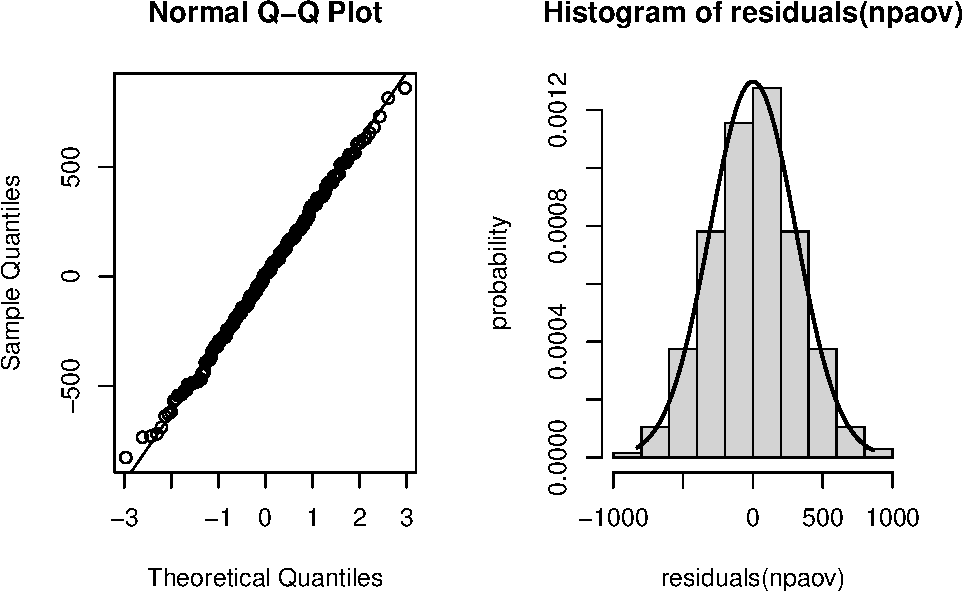
\includegraphics{AEII_main_files/figure-latex/unnamed-chunk-6-1.pdf}

\begin{Shaded}
\begin{Highlighting}[]
\CommentTok{\# voltar ao layout grafico normal}
\FunctionTok{par}\NormalTok{(}\AttributeTok{mfrow =} \FunctionTok{c}\NormalTok{(}\DecValTok{1}\NormalTok{, }\DecValTok{1}\NormalTok{))}
\end{Highlighting}
\end{Shaded}

Como se pode observar em ambos os gráficos, os resíduos da amostra
exibem uma grande proximidade em relação às linhas que representam a
distribuição normal, pelo que será de esperar que os resíduos sigam uma
distribuição normal.

Para corroborar esta observação, de forma a obtermos uma validação mais
formal da normalidade dos resíduos, devemos realizar o teste de
normalidade de Shapiro-Wilk. \[
H_0:\ Os\ residuos\ seguem\ uma\ distribuic\tilde{a}o\ normal\
vs\
H_1:\ Os\ residuos\ n\tilde{a}o\ seguem\ uma\ distribuic\tilde{a}o\ normal
\]

\begin{Shaded}
\begin{Highlighting}[]
\FunctionTok{shapiro.test}\NormalTok{(}\FunctionTok{residuals}\NormalTok{(npaov))}
\end{Highlighting}
\end{Shaded}

\begin{verbatim}
## 
##  Shapiro-Wilk normality test
## 
## data:  residuals(npaov)
## W = 0.99776, p-value = 0.9367
\end{verbatim}

\(p-value = 0.9367 > 0.05 = \alpha\ \Rightarrow\ \) não rejeitamos
\(H_0\) para o nível de significância de 5\%, isto é, existe evidência
estatística dos resíduos da amostra seguirem uma distribuição normal.

\(\ \)

Para além da análise da normalidade dos resíduos, também é importante
testar a normalidade das observações. Com este propósito, devemos
realizar testes de Shapiro-Wilk entre cada grupo de observações, ou
seja, um teste para cada combinação entre \emph{species} e \emph{sex},
dado que são estas as variáveis explicativas.
\[ H_0:\ O\ grupo_{species,sex}\ segue\ uma\ distribuic\tilde{a}o\ normal\]
\[ H_1:\ O\ grupo_{species,sex}\ n\tilde{a}o\ segue\ uma\ distribuic\tilde{a}o\ normal\]

\begin{Shaded}
\begin{Highlighting}[]
\FunctionTok{aggregate}\NormalTok{(body\_mass\_g }\SpecialCharTok{\textasciitilde{}}\NormalTok{ species }\SpecialCharTok{*}\NormalTok{ sex, }\AttributeTok{data =}\NormalTok{ peng\_clean,}
          \ControlFlowTok{function}\NormalTok{(x) }\FunctionTok{shapiro.test}\NormalTok{(x)}\SpecialCharTok{$}\NormalTok{p.value)}
\end{Highlighting}
\end{Shaded}

\begin{verbatim}
##     species    sex body_mass_g
## 1    Adelie female   0.1985303
## 2 Chinstrap female   0.3055292
## 3    Gentoo female   0.5106595
## 4    Adelie   male   0.4159824
## 5 Chinstrap   male   0.8910238
## 6    Gentoo   male   0.9850457
\end{verbatim}

\(min\{p-value_{species,sex}\} \approx 0.1985 > 0.05 = \alpha\ \Rightarrow\ \)
não rejeitamos nenhum dos \(H_0\) para o nível de significância de 5\%,
isto é, existe evidência estatística de que todos os grupos seguem uma
distribuição normal.

\(\ \)

Desta forma, após termos analisado os resultados dos testes de
Shapiro-Wilk, podemos concluir que tanto os resíduos como as observações
seguem distribuições normais, pelo que esta constatação valida a
pressuposição de normalidade.

\subsubsection{Independência dos resíduos}

Após a análise do pressuposto da normalidade, devemos analisar a
validade do pressuposto da independência, isto é, devemos agora
verificar se os resíduos são independentes entre si. Com este objetivo,
vamos analisar a independência resíduos através de uma abordagem visual.

\begin{Shaded}
\begin{Highlighting}[]
\FunctionTok{plot}\NormalTok{(}\FunctionTok{residuals}\NormalTok{(npaov), }\AttributeTok{ylab =} \StringTok{"Residuals"}\NormalTok{, }\AttributeTok{xlab =} \StringTok{"Observation Index"}\NormalTok{,}
     \AttributeTok{main =} \StringTok{"Residuals Plot for ANOVA"}\NormalTok{)}
\end{Highlighting}
\end{Shaded}

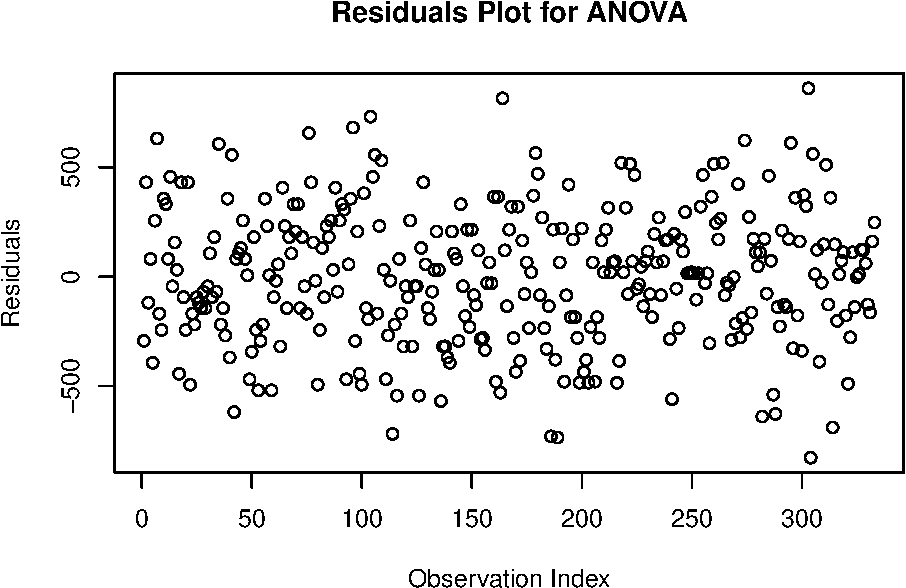
\includegraphics{AEII_main_files/figure-latex/unnamed-chunk-9-1.pdf}

Através da visualização do gráfico dos resíduos, podemos verificar que
não existe qualquer padrão entre os mesmos, mas sim uma distribuição
aleatória entre eles, ao longo do eixo horizontal, o que nos permite
concluir que há independência dos resíduos, ou seja, verifica-se o
pressuposto.

\subsubsection{Homogeneidade das variâncias}

Atendendo ao pressuposto que nos falta verificar, a homogeneidade das
variâncias, este pode ser analisado de forma gráfica, através da análise
da relação entre os resíduos e os valores ajustados, e também através da
realização de um teste estatístico, o teste de Bartlett.

Comecemos pela forma gráfica.

\begin{Shaded}
\begin{Highlighting}[]
\FunctionTok{par}\NormalTok{(}\AttributeTok{mfrow =} \FunctionTok{c}\NormalTok{(}\DecValTok{1}\NormalTok{, }\DecValTok{2}\NormalTok{))}

\CommentTok{\# dispersao entre valores ajustados e residuos}
\FunctionTok{plot}\NormalTok{(}\FunctionTok{fitted}\NormalTok{(npaov), }\FunctionTok{residuals}\NormalTok{(npaov), }\AttributeTok{col =} \StringTok{"darkgray"}\NormalTok{, }\AttributeTok{pch =} \DecValTok{10}\NormalTok{)}
\CommentTok{\# linha que melhor se ajusta aos padroes dos residuos}
\FunctionTok{lines}\NormalTok{(}\FunctionTok{lowess}\NormalTok{(}\FunctionTok{residuals}\NormalTok{(npaov) }\SpecialCharTok{\textasciitilde{}} \FunctionTok{fitted}\NormalTok{(npaov)), }\AttributeTok{col =} \StringTok{"black"}\NormalTok{)}

\CommentTok{\# aplicar transformacao logaritmica para tornar padroes mais evidentes}
\NormalTok{log\_resid }\OtherTok{\textless{}{-}} \FunctionTok{log1p}\NormalTok{(}\FunctionTok{abs}\NormalTok{(}\FunctionTok{residuals}\NormalTok{(npaov)))}
\FunctionTok{plot}\NormalTok{(}\FunctionTok{fitted}\NormalTok{(npaov), log\_resid, }\AttributeTok{col =} \StringTok{"darkgray"}\NormalTok{, }\AttributeTok{pch =} \DecValTok{10}\NormalTok{)}
\FunctionTok{lines}\NormalTok{(}\FunctionTok{lowess}\NormalTok{(log\_resid }\SpecialCharTok{\textasciitilde{}} \FunctionTok{fitted}\NormalTok{(npaov)), }\AttributeTok{col =} \StringTok{"black"}\NormalTok{)}
\end{Highlighting}
\end{Shaded}

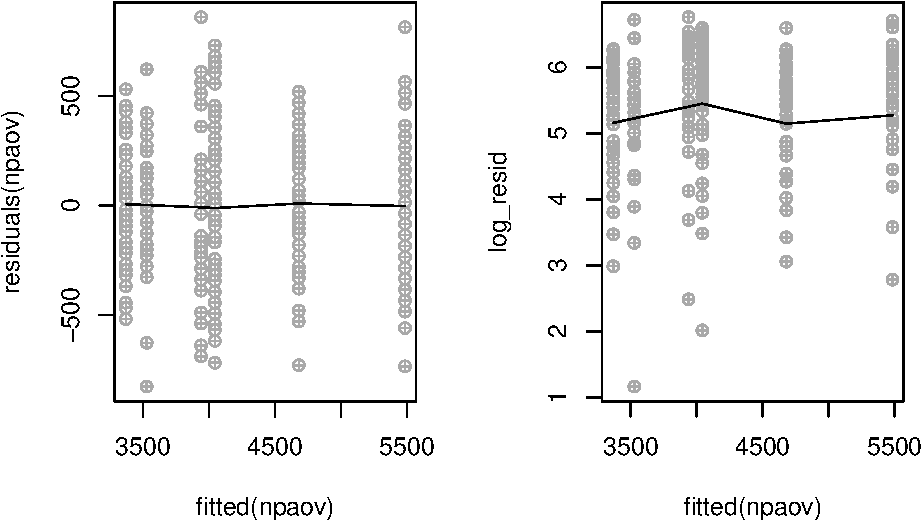
\includegraphics{AEII_main_files/figure-latex/unnamed-chunk-10-1.pdf}

\begin{Shaded}
\begin{Highlighting}[]
\FunctionTok{par}\NormalTok{(}\AttributeTok{mfrow =} \FunctionTok{c}\NormalTok{(}\DecValTok{1}\NormalTok{, }\DecValTok{1}\NormalTok{))}
\end{Highlighting}
\end{Shaded}

Pelo facto da linha que melhor se ajusta à dispersão dos resíduos ser
significativamente horizontal, pode-se verificar que a dispersão dos
mesmos é constante, pelo que o pressuposto da homogeneidade de
variâncias se verifica.

De qualquer forma, analisemos agora o pressuposto, novamente, mas
através do teste de Bartlett.

\begin{Shaded}
\begin{Highlighting}[]
\FunctionTok{detach}\NormalTok{(peng\_clean)}
\CommentTok{\# introduzir coluna nova do tipo "species.sex" (ex.: Gentoo.female)}
\NormalTok{peng\_clean}\SpecialCharTok{$}\NormalTok{bart }\OtherTok{\textless{}{-}} \FunctionTok{interaction}\NormalTok{(peng\_clean}\SpecialCharTok{$}\NormalTok{species, peng\_clean}\SpecialCharTok{$}\NormalTok{sex)}
\FunctionTok{attach}\NormalTok{(peng\_clean)}

\FunctionTok{summary}\NormalTok{(bart)}
\end{Highlighting}
\end{Shaded}

\begin{verbatim}
##    Adelie.female Chinstrap.female    Gentoo.female      Adelie.male 
##               73               34               58               73 
##   Chinstrap.male      Gentoo.male 
##               34               61
\end{verbatim}

Note-se que todos os grupos têm pelo menos 5 observações, pelo que os
resultados serão mais significantes, dada a sensibilidade deste teste ao
tamanho das amostras. Avancemos com o teste. \[
H_0:\ \exists\ homogeneidade\ de\ vari\hat{a}ncias\
vs\
H_1:\ \nexists\ existe\ homogeneidade\ de \ vari\hat{a}ncias
\]

\begin{Shaded}
\begin{Highlighting}[]
\FunctionTok{bartlett.test}\NormalTok{(body\_mass\_g }\SpecialCharTok{\textasciitilde{}}\NormalTok{ bart, }\AttributeTok{data =}\NormalTok{ peng\_clean)}
\end{Highlighting}
\end{Shaded}

\begin{verbatim}
## 
##  Bartlett test of homogeneity of variances
## 
## data:  body_mass_g by bart
## Bartlett's K-squared = 7.6908, df = 5, p-value = 0.1741
\end{verbatim}

\(p-value = 0.1741 > 0.05 = \alpha\ \Rightarrow\ \) não rejeitamos
\(H_0\) para o nível de significância de 5\%, isto é, existe evidência
estatística de não haverem diferenças significativas entre as variâncias
de diferentes grupos. Assim, verifica-se o pressuposto da homogeneidade
das variâncias, tal como já havíamos verificado anteriormente.

\begin{Shaded}
\begin{Highlighting}[]
\FunctionTok{detach}\NormalTok{(peng\_clean)}
\end{Highlighting}
\end{Shaded}

Em suma, tendo por base as análises realizadas, verificamos que os dados
atendem aos pressupostos desejados, o que fortalece a validade
estatística dos próprios, estabelecendo uma base sólida e confiável para
a interpretação dos resultados subsequentes da análise de variância,
assegurando a robustez e a precisão das conclusões extraídas a partir
desse estudo.

\subsection{Análise descritiva dos dados}

Realizada a verificação dos pressupostos para o nosso conjunto de dados,
estamos prontos para realizar uma análise descritiva. Isto implica
calcular as médias por variável (\emph{species} e \emph{sex}) e por
grupo formado pela combinação das mesmas (\emph{species.sex}), o que nos
irá permitir ter uma perceção dos resultados que devemos esperar ao
realizar a análise de variância. Para além do cálculo das médias, também
podemos criar gráficos de interação, de modo a observar a presença, ou
não, de interação entre os fatores.

\(\ \)

Comecemos pelo cálculo das médias por variável, mas ao invés de nos
restringirmos a números, exploremos visualmente as mesmas.

\begin{Shaded}
\begin{Highlighting}[]
\FunctionTok{attach}\NormalTok{(peng\_clean)}
\FunctionTok{par}\NormalTok{(}\AttributeTok{mfrow =} \FunctionTok{c}\NormalTok{(}\DecValTok{1}\NormalTok{, }\DecValTok{2}\NormalTok{))}

\CommentTok{\# media species e sex, atraves de caixas de bigodes}
\FunctionTok{plot}\NormalTok{(species, body\_mass\_g, }\AttributeTok{ylab =} \StringTok{"body\_mass\_g"}\NormalTok{, }\AttributeTok{xlab =} \StringTok{"species"}\NormalTok{, }\AttributeTok{cex.axis =} \FloatTok{0.7}\NormalTok{)}
\FunctionTok{plot}\NormalTok{(sex, body\_mass\_g, }\AttributeTok{ylab =} \StringTok{"body\_mass\_g"}\NormalTok{, }\AttributeTok{xlab =} \StringTok{"sex"}\NormalTok{, }\AttributeTok{cex.axis =} \FloatTok{0.7}\NormalTok{)}
\end{Highlighting}
\end{Shaded}

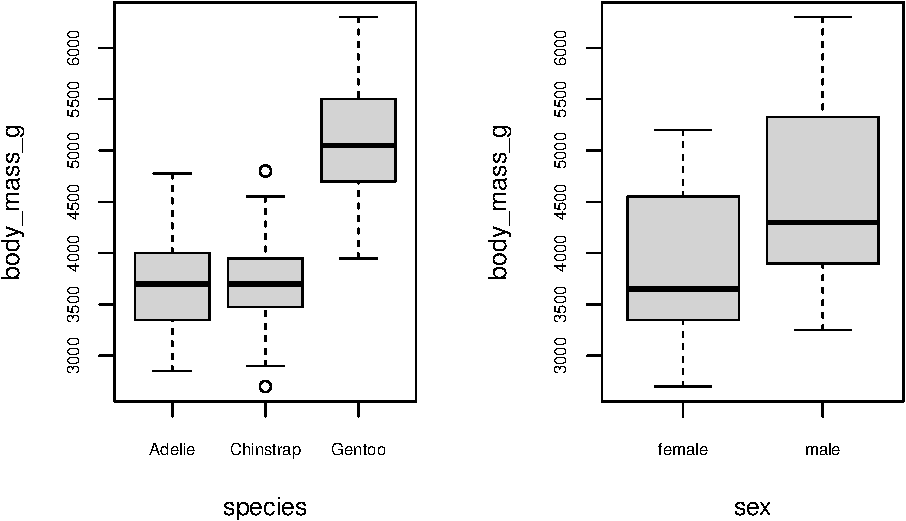
\includegraphics{AEII_main_files/figure-latex/unnamed-chunk-14-1.pdf}

\begin{Shaded}
\begin{Highlighting}[]
\FunctionTok{par}\NormalTok{(}\AttributeTok{mfrow =} \FunctionTok{c}\NormalTok{(}\DecValTok{1}\NormalTok{, }\DecValTok{1}\NormalTok{))}
\end{Highlighting}
\end{Shaded}

Note-se que apenas não há diferenças significativas entre as médias das
espécies Adelie e Chinstrap, pelo que será de esperar que rejeitemos a
hipótese de haver igualdade entre as médias tanto na variável
\emph{species}, como na variável \emph{sex}.

\(\ \)

Analisemos agora as médias entre os grupos formados por cada tipo de
\emph{species} e \emph{sex}.

\begin{Shaded}
\begin{Highlighting}[]
\CommentTok{\# media species.sex}
\FunctionTok{aggregate}\NormalTok{(body\_mass\_g }\SpecialCharTok{\textasciitilde{}}\NormalTok{ species }\SpecialCharTok{*}\NormalTok{ sex, }\AttributeTok{data =}\NormalTok{ peng\_clean, }\AttributeTok{FUN =}\NormalTok{ mean)}
\end{Highlighting}
\end{Shaded}

\begin{verbatim}
##     species    sex body_mass_g
## 1    Adelie female    3368.836
## 2 Chinstrap female    3527.206
## 3    Gentoo female    4679.741
## 4    Adelie   male    4043.493
## 5 Chinstrap   male    3938.971
## 6    Gentoo   male    5484.836
\end{verbatim}

Como podemos verificar, a análise das diferenças entre as médias de
forma numérica é mais trabalhosa do que através de representações
gráficas. Contudo, podemos, ainda assim, observar que apenas há
proximidade nas médias entre as espécies Adelie e Chinstrap, quando
ambos são ou machos ou fêmeas.

\(\ \)

No que diz respeito à interação entre os fatores, procederemos à criação
de gráficos de interação para verificar a existência, ou não, da mesma,
tal como referido.

\begin{Shaded}
\begin{Highlighting}[]
\FunctionTok{par}\NormalTok{(}\AttributeTok{mfrow =} \FunctionTok{c}\NormalTok{(}\DecValTok{1}\NormalTok{, }\DecValTok{2}\NormalTok{))}
\CommentTok{\# mudar tamanho da fonte (lab, axis, tudo) em \%}
\FunctionTok{par}\NormalTok{(}\AttributeTok{cex.lab =} \FloatTok{1.3}\NormalTok{, }\AttributeTok{cex.axis =} \FloatTok{1.3}\NormalTok{, }\AttributeTok{cex=}\FloatTok{0.6}\NormalTok{)}

\CommentTok{\# fazer os graficos de interacao}
\FunctionTok{with}\NormalTok{(peng\_clean, }\FunctionTok{interaction.plot}\NormalTok{(species, sex, body\_mass\_g,}
                           \AttributeTok{type =} \StringTok{"b"}\NormalTok{, }\AttributeTok{pch =} \DecValTok{19}\NormalTok{, }\AttributeTok{fixed =}\NormalTok{ T,}
                           \AttributeTok{xlab =} \StringTok{"species"}\NormalTok{, }\AttributeTok{ylab =} \StringTok{"media body\_mass\_g"}\NormalTok{, }\AttributeTok{legend =} \ConstantTok{FALSE}\NormalTok{))}
\FunctionTok{legend}\NormalTok{(}\StringTok{"bottomright"}\NormalTok{, }\AttributeTok{legend =} \FunctionTok{c}\NormalTok{(}\StringTok{"female"}\NormalTok{, }\StringTok{"male"}\NormalTok{),}
       \AttributeTok{title =} \StringTok{"species"}\NormalTok{, }\AttributeTok{lty =} \FunctionTok{c}\NormalTok{(}\DecValTok{2}\NormalTok{,}\DecValTok{1}\NormalTok{), }\AttributeTok{pch =} \DecValTok{19}\NormalTok{)}

\FunctionTok{with}\NormalTok{(peng\_clean, }\FunctionTok{interaction.plot}\NormalTok{(sex, species, body\_mass\_g,}
                                  \AttributeTok{type =} \StringTok{"b"}\NormalTok{, }\AttributeTok{pch =} \DecValTok{19}\NormalTok{, }\AttributeTok{fixed =}\NormalTok{ T,}
                                  \AttributeTok{xlab =} \StringTok{"sex"}\NormalTok{, }\AttributeTok{ylab =} \StringTok{"media body\_mass\_g"}\NormalTok{, }\AttributeTok{legend =} \ConstantTok{FALSE}\NormalTok{))}
\FunctionTok{legend}\NormalTok{(}\StringTok{"bottomright"}\NormalTok{, }\AttributeTok{legend =} \FunctionTok{c}\NormalTok{(}\StringTok{"Adelie"}\NormalTok{, }\StringTok{"Chinstrap"}\NormalTok{, }\StringTok{"Gentoo"}\NormalTok{),}
       \AttributeTok{title =} \StringTok{"sex"}\NormalTok{, }\AttributeTok{lty =} \FunctionTok{c}\NormalTok{(}\DecValTok{3}\NormalTok{,}\DecValTok{2}\NormalTok{,}\DecValTok{1}\NormalTok{), }\AttributeTok{pch =} \DecValTok{19}\NormalTok{)}
\end{Highlighting}
\end{Shaded}

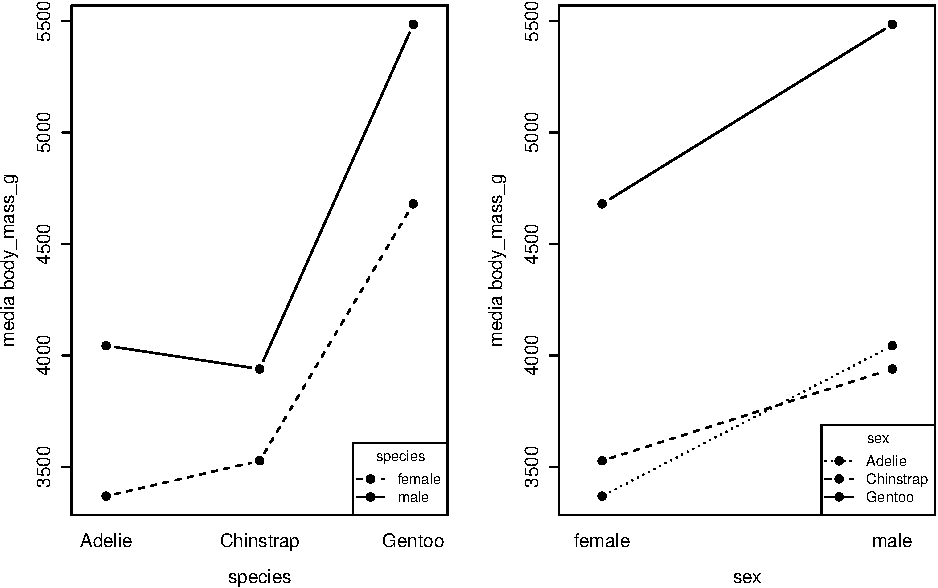
\includegraphics{AEII_main_files/figure-latex/unnamed-chunk-16-1.pdf}

\begin{Shaded}
\begin{Highlighting}[]
\FunctionTok{par}\NormalTok{(}\AttributeTok{mfrow =} \FunctionTok{c}\NormalTok{(}\DecValTok{1}\NormalTok{, }\DecValTok{1}\NormalTok{))}
\FunctionTok{detach}\NormalTok{(peng\_clean)}
\end{Highlighting}
\end{Shaded}

Como podemos observar, no primeiro gráfico, há falta de paralelismo. O
mesmo se passa no segundo gráfico, de forma ainda mais evidente, pelo
facto de haver interseção de duas retas. Estas observações indicam-nos
que haverá interação entre os fatores.

\subsection{Análise de variância (ANOVA)}

Finalmente, após o tratamento dos dados, a verificação dos pressupostos
e uma breve análise descritiva, podemos realizar a análise de variância
(ANOVA). Esta análise permite-nos testar as seguintes hipóteses:

\begin{itemize}
  \item $H_0':\ \mu_{Adelie}=\mu_{Chinstrap}=\mu_{Gentoo}=\mu\ vs\ H_1':\ \exists_{i}:\  \mu_{i} \neq \mu$

  \item $H_0'':\ \mu_{female}=\mu_{male}=\mu\ vs\ H_1'':\ \exists_{j}:\  \mu_{j} \neq \mu$

  \item $H_0''':\ \nexists\ interac\tilde{a}o\ entre\ os\ fatores\ species\ e\ sex\ vs\ H_1''':\ \exists\ interac\tilde{a}o\ entre\ os\ fatores\ species\ e\ sex$
\end{itemize}

\begin{Shaded}
\begin{Highlighting}[]
\FunctionTok{summary}\NormalTok{(npaov)}
\end{Highlighting}
\end{Shaded}

\begin{verbatim}
##              Df    Sum Sq  Mean Sq F value   Pr(>F)    
## species       2 145190219 72595110 758.358  < 2e-16 ***
## sex           1  37090262 37090262 387.460  < 2e-16 ***
## species:sex   2   1676557   838278   8.757 0.000197 ***
## Residuals   327  31302628    95727                     
## ---
## Signif. codes:  0 '***' 0.001 '**' 0.01 '*' 0.05 '.' 0.1 ' ' 1
\end{verbatim}

Comecemos por analisar a interação entre os fatores:

\(p-value = 0.000197 < 0.05 = \alpha\ \Rightarrow\ \) rejeitamos
\(H_0'''\) para o nível de significância de 5\%, isto é, existe
evidência estatística de haver interação significativa entre os fatores
\emph{species} e \emph{sex}, tal como já havíamos previsto na análise
descritiva.

\(\ \)

De seguida, analisemos os níveis médios do fator \emph{species}:

\(p-value < 2e-16 < 0.05 = \alpha\ \Rightarrow\ \) rejeitamos \(H_0'\)
para o nível de significância de 5\%, isto é, existe evidência
estatística de haver diferenças significativas entre o peso médio dos
pinguins para os níveis do fator \emph{species}, quando considerados
relativamente aos níveis do fator \emph{sex}, em média.

\(\ \)

E por último, analisemos os níveis médios do fator \emph{sex}:

\(p-value < 2e-16 < 0.05 = \alpha\ \Rightarrow\ \) rejeitamos \(H_0''\)
para o nível de significância de 5\%, isto é, existe evidência
estatística de haver diferenças significativas entre o peso médio dos
pinguins para os níveis do fator \emph{sex}, quando considerados
relativamente aos níveis do fator \emph{species}, em média.

\(\ \)

Pelo facto de termos verificado que existem diferenças entre o peso
médio dos pinguins, tanto para os níveis do fator \emph{species}, como
para os níveis do fator \emph{sex}, tal como era de esperar, tendo em
conta as conclusões tiradas a partir da análise descritiva, temos agora
de averiguar que grupos (\emph{species:sex}, dado que os fatores têm
interação) têm, ou não, médias significativamente diferentes. Para
realizar estas comparações múltiplas iremos utilizar o teste de Tukey,
tanto numérica como graficamente. \[
H_0:\ \mu_{species_i,sex_i}=\mu_{species_j,sex_j}\
vs\
H_1:\ \mu_{species_i,sex_i}\neq\mu_{species_j,sex_j}
\]

\begin{Shaded}
\begin{Highlighting}[]
\FunctionTok{TukeyHSD}\NormalTok{(npaov, }\StringTok{"species:sex"}\NormalTok{)}
\end{Highlighting}
\end{Shaded}

\begin{verbatim}
##   Tukey multiple comparisons of means
##     95% family-wise confidence level
## 
## Fit: aov(formula = body_mass_g ~ species * sex, data = peng_clean)
## 
## $`species:sex`
##                                      diff       lwr       upr     p adj
## Chinstrap:female-Adelie:female   158.3703  -25.7874  342.5279 0.1376213
## Gentoo:female-Adelie:female     1310.9058 1154.8934 1466.9181 0.0000000
## Adelie:male-Adelie:female        674.6575  527.8486  821.4664 0.0000000
## Chinstrap:male-Adelie:female     570.1350  385.9773  754.2926 0.0000000
## Gentoo:male-Adelie:female       2116.0004 1962.1408 2269.8601 0.0000000
## Gentoo:female-Chinstrap:female  1152.5355  960.9603 1344.1107 0.0000000
## Adelie:male-Chinstrap:female     516.2873  332.1296  700.4449 0.0000000
## Chinstrap:male-Chinstrap:female  411.7647  196.6479  626.8815 0.0000012
## Gentoo:male-Chinstrap:female    1957.6302 1767.8040 2147.4564 0.0000000
## Adelie:male-Gentoo:female       -636.2482 -792.2606 -480.2359 0.0000000
## Chinstrap:male-Gentoo:female    -740.7708 -932.3460 -549.1956 0.0000000
## Gentoo:male-Gentoo:female        805.0947  642.4300  967.7594 0.0000000
## Chinstrap:male-Adelie:male      -104.5226 -288.6802   79.6351 0.5812048
## Gentoo:male-Adelie:male         1441.3429 1287.4832 1595.2026 0.0000000
## Gentoo:male-Chinstrap:male      1545.8655 1356.0392 1735.6917 0.0000000
\end{verbatim}

Tendo em conta o teste de Tukey realizado, podemos reparar que apenas as
combinações \textit{Chinstrap:female-Adelie:female} e
\textit{Chinstrap:male−Adelie:male} têm p-values superiores a 0.05
(0.1376213 e 0.5812048, respetivamente), pelo que as restantes
combinações de grupos rejeitam \(H_0\), mas estas não. Isto significa
que para um nível de significância de 5\%, existe evidência estatística
de que os pinguins fêmea das espécies Chinstrap e Adelie não têm
diferenças significativas no seu peso médio, tal como os pinguins machos
das mesmas espécies, e de que os pesos médios dos restantes grupos de
pinguins (\emph{species:sex}) têm todos diferenças significativas entre
si.

\begin{Shaded}
\begin{Highlighting}[]
\CommentTok{\# alterar as margens (baixo, esqueda, cima, direita)}
\FunctionTok{par}\NormalTok{(}\AttributeTok{mar =} \FunctionTok{c}\NormalTok{(}\DecValTok{4}\NormalTok{, }\DecValTok{9}\NormalTok{, }\DecValTok{2}\NormalTok{, }\DecValTok{0}\NormalTok{))}
\FunctionTok{plot}\NormalTok{(}\FunctionTok{TukeyHSD}\NormalTok{(npaov, }\StringTok{"species:sex"}\NormalTok{), }\AttributeTok{cex.axis =} \FloatTok{0.6}\NormalTok{, }\AttributeTok{las =} \DecValTok{1}\NormalTok{)}
\end{Highlighting}
\end{Shaded}

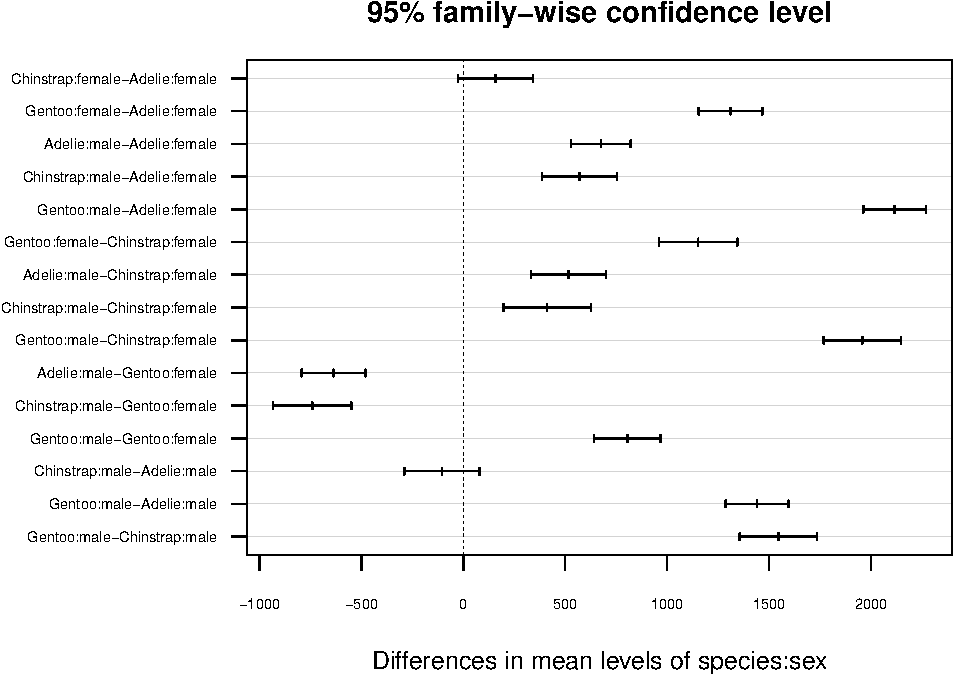
\includegraphics{AEII_main_files/figure-latex/unnamed-chunk-19-1.pdf}

Através da análise do gráfico, chegamos às mesmas conclusões mencionadas
anteriormente. As combinações que incluem o valor zero no seu intervalo
são aquelas que provam estatisticamente a ausência de diferenças
significativas entre os pesos médios entre os grupos de pinguins a serem
comparados. Isto é, as combinações que contêm o valor zero no seu
intervalo, são aquelas que não rejeitam a hipótese nula (\(H_0\))
definida anteriormente, enquanto que as restantes a rejeitam.

\(\ \)

Note-se que todas as conclusões derivadas da análise de variância já
haviam sido antecipadas durante a análise descritiva, evidenciando,
desta forma, concordância entre as previsões e as conclusões, como seria
de esperar.

\newpage
\section{Exercício 2}

\textit{O conjunto de dados “sat” do package “faraway” foi obtido com o objetivo de estudar
a relação entre as despesas dos alunos com a educação no ensino público e os resultados
obtidos no exame SAT.}

\begin{Shaded}
\begin{Highlighting}[]
\FunctionTok{library}\NormalTok{(faraway)}
\FunctionTok{head}\NormalTok{(sat, }\DecValTok{12}\NormalTok{)}
\end{Highlighting}
\end{Shaded}

\begin{verbatim}
##             expend ratio salary takers verbal math total
## Alabama      4.405  17.2 31.144      8    491  538  1029
## Alaska       8.963  17.6 47.951     47    445  489   934
## Arizona      4.778  19.3 32.175     27    448  496   944
## Arkansas     4.459  17.1 28.934      6    482  523  1005
## California   4.992  24.0 41.078     45    417  485   902
## Colorado     5.443  18.4 34.571     29    462  518   980
## Connecticut  8.817  14.4 50.045     81    431  477   908
## Delaware     7.030  16.6 39.076     68    429  468   897
## Florida      5.718  19.1 32.588     48    420  469   889
## Georgia      5.193  16.3 32.291     65    406  448   854
## Hawaii       6.078  17.9 38.518     57    407  482   889
## Idaho        4.210  19.1 29.783     15    468  511   979
\end{verbatim}

O conjunto de dados contém 7 variáveis relativas aos resultados de 50
alunos. No entanto, para a nossa regressão linear múltipla, apenas
iremos considerar as variáveis despesas (\emph{expend}), razão média de
alunos por professor (\emph{ratio}), ordenado (\emph{salary}),
percentagem de alunos elegíveis para fazerem o exame (\emph{takers}) e
pontuação média total no SAT (\emph{total}).

Para simplificar o conjunto de dados, podemos criar um novo DataFrame,
apenas com as variáveis necessárias.

\begin{Shaded}
\begin{Highlighting}[]
\NormalTok{sat\_clean }\OtherTok{\textless{}{-}}\NormalTok{ sat[, }\FunctionTok{c}\NormalTok{(}\StringTok{"total"}\NormalTok{, }\StringTok{"expend"}\NormalTok{, }\StringTok{"ratio"}\NormalTok{, }\StringTok{"salary"}\NormalTok{, }\StringTok{"takers"}\NormalTok{)]}
\FunctionTok{head}\NormalTok{(sat\_clean, }\DecValTok{12}\NormalTok{)}
\end{Highlighting}
\end{Shaded}

\begin{verbatim}
##             total expend ratio salary takers
## Alabama      1029  4.405  17.2 31.144      8
## Alaska        934  8.963  17.6 47.951     47
## Arizona       944  4.778  19.3 32.175     27
## Arkansas     1005  4.459  17.1 28.934      6
## California    902  4.992  24.0 41.078     45
## Colorado      980  5.443  18.4 34.571     29
## Connecticut   908  8.817  14.4 50.045     81
## Delaware      897  7.030  16.6 39.076     68
## Florida       889  5.718  19.1 32.588     48
## Georgia       854  5.193  16.3 32.291     65
## Hawaii        889  6.078  17.9 38.518     57
## Idaho         979  4.210  19.1 29.783     15
\end{verbatim}

\subsection{Estimação do modelo de regressão linear múltipla}

Após termos selecionado as variáveis que vamos utilizar, podemos agora
construir o nosso modelo de regressão linear múltipla, o que nos irá
permitir explorar a relação entre as variáveis explicativas
(\emph{expend}, \emph{ratio}, \emph{salary}, \emph{takers}) e a variável
dependente (\emph{total}).

\begin{Shaded}
\begin{Highlighting}[]
\CommentTok{\# criar o modelo de regressao linear}
\NormalTok{sat\_lm }\OtherTok{\textless{}{-}} \FunctionTok{lm}\NormalTok{(total }\SpecialCharTok{\textasciitilde{}}\NormalTok{ expend }\SpecialCharTok{+}\NormalTok{ ratio }\SpecialCharTok{+}\NormalTok{ salary }\SpecialCharTok{+}\NormalTok{ takers, }\AttributeTok{data =}\NormalTok{ sat\_clean)}
\NormalTok{sat\_lm}
\end{Highlighting}
\end{Shaded}

\begin{verbatim}
## 
## Call:
## lm(formula = total ~ expend + ratio + salary + takers, data = sat_clean)
## 
## Coefficients:
## (Intercept)       expend        ratio       salary       takers  
##    1045.972        4.463       -3.624        1.638       -2.904
\end{verbatim}

Estimado o modelo, devemos analisar os coeficientes, ou seja, vamos
verificar o impacto de cada variável explicativa na variável dependente
e analisar o que significa esse impacto no contexto dos nossos dados.

\begin{itemize}
  \item $\beta_0:$ Estima-se que se todas as variáveis explicativas (\textit{expend},
\textit{ratio}, \textit{salary} e \textit{takers}) forem nulas, então a pontuação
média total no SAT (\textit{total}) será de 1045.9715 unidades.
  
  \item $\beta_{expend}:$ Estima-se que por cada variação unitária nas despesas
(\textit{expend}), a pontuação média total no SAT (\textit{total}) varie 4.4626 unidades,
assumindo tudo o resto constante.
  
  \item $\beta_{ratio}:$ Estima-se que por cada variação unitária na razão média
de alunos por professor (\textit{ratio}), a pontuação média total no SAT
(\textit{total}) varie -3.6242 unidades, assumindo tudo o resto constante.
  
  \item $\beta_{salary}:$ Estima-se que por cada variação unitária no ordenado
(\textit{salary}), a pontuação média total no SAT (\textit{total}) varie 1.6379 unidades,
assumindo tudo o resto constante.
  
  \item $\beta_{takers}:$ Estima-se que por cada variação unitária na percentagem
de alunos elegíveis para fazerem o exame (\textit{takers}), a pontuação média total
no SAT (\textit{total}) varie -2.9045 unidades, assumindo tudo o resto constante.
\end{itemize}

\subsection{Interpretação do modelo estimado}

Tendo em conta o modelo de regressão estimado, através da análise do
mesmo, para além de podermos interpretar os coeficientes, tal como
fizemos, podemos interpretar outros valores, o que nos irá permitir
tirar outras conlusões sobre o modelo.

\begin{Shaded}
\begin{Highlighting}[]
\FunctionTok{summary}\NormalTok{(sat\_lm)}
\end{Highlighting}
\end{Shaded}

\begin{verbatim}
## 
## Call:
## lm(formula = total ~ expend + ratio + salary + takers, data = sat_clean)
## 
## Residuals:
##     Min      1Q  Median      3Q     Max 
## -90.531 -20.855  -1.746  15.979  66.571 
## 
## Coefficients:
##              Estimate Std. Error t value Pr(>|t|)    
## (Intercept) 1045.9715    52.8698  19.784  < 2e-16 ***
## expend         4.4626    10.5465   0.423    0.674    
## ratio         -3.6242     3.2154  -1.127    0.266    
## salary         1.6379     2.3872   0.686    0.496    
## takers        -2.9045     0.2313 -12.559 2.61e-16 ***
## ---
## Signif. codes:  0 '***' 0.001 '**' 0.01 '*' 0.05 '.' 0.1 ' ' 1
## 
## Residual standard error: 32.7 on 45 degrees of freedom
## Multiple R-squared:  0.8246, Adjusted R-squared:  0.809 
## F-statistic: 52.88 on 4 and 45 DF,  p-value: < 2.2e-16
\end{verbatim}

Comecemos por analisar os resultados presentes sobre os testes de
significância individuais: \[
H_0:\ \beta_i=0\
vs\
H_1:\ \beta_i \neq 0
\]

\begin{itemize}
  \item $\beta_{expend}:$ $p-value = 0.674 > 0.05 = \alpha\ \Rightarrow\ $ não
rejeitamos $H_0$ para o nível de significância de 5\%, isto é, existe envidência
estatística de que a variável \textit{expend} não é significativa para o modelo
que inclui as variáveis \textit{ratio}, \textit{salary} e \textit{takers}.
  
  \item $\beta_{ratio}:$ $p-value = 0.266 > 0.05 = \alpha\ \Rightarrow\ $ não
rejeitamos $H_0$ para o nível de significância de 5\%, isto é, existe envidência
estatística de que a variável \textit{ratio} não é significativa para o modelo
que inclui as variáveis \textit{expend}, \textit{salary} e \textit{takers}.
  
  \item $\beta_{salary}:$ $p-value = 0.496 > 0.05 = \alpha\ \Rightarrow\ $ não
rejeitamos $H_0$ para o nível de significância de 5\%, isto é, existe envidência
estatística de que a variável \textit{salary} não é significativa para o modelo
que inclui as variáveis \textit{expend}, \textit{ratio} e \textit{takers}.
  
  \item $\beta_{takers}:$ $p-value = 2.61e-16 < 0.05 = \alpha\ \Rightarrow\ $ rejeitamos
$H_0$ para o nível de significância de 5\%, isto é, existe envidência estatística de que
a variável \textit{takers} é significativa para o modelo que inclui as variáveis
\textit{expend}, \textit{ratio} e \textit{salary}.
  
\end{itemize}

\(\ \)

De seguida, podemos verificar que \emph{Adjusted R-squared: 0.809}, o
que nos indica que aproximadamente 81\% da variação da pontuação média
total no SAT (\emph{total}), pode ser explicada pelo modelo estimado.

\(\ \)

Por último, também é de elevada importância avaliar a significância do
modelo de regressão linear múltipla estimado: \[
H_0:\ \beta_0=\beta_{expend}=\beta_{ratio}=\beta_{salary}=\beta_{takers}=0\
vs\
H_1:\ \exists_i:\beta_i \neq 0
\]

\(p-value < 2.2e-16 < 0.05 = \alpha\ \Rightarrow\ \) rejeitamos \(H_0\)
para o nível de significância de 5\%, isto é, existe evidência
estatística de que o modelo ajustado é significativo, ou seja, pelo
menos uma das variáveis explicativas tem um efeito significativo sobre a
variável dependente.

\subsection{Análise de resíduos}

Antes de mais, devemos avaliar determinadas suposições sobre o nosso
conjunto de dados, ver se as mesmas se verificam. Se as suposições da
regressão se mantiverem, os resíduos deverão ser normalmente
distribuídos, com valor médio zero e variância constante e independentes
entre si.

\(\ \)

Comecemos por verificar se são normalmente distribuídos:

\begin{Shaded}
\begin{Highlighting}[]
\FunctionTok{par}\NormalTok{(}\AttributeTok{mfrow =} \FunctionTok{c}\NormalTok{(}\DecValTok{1}\NormalTok{,}\DecValTok{2}\NormalTok{))}

\CommentTok{\# grafico qq}
\FunctionTok{qqnorm}\NormalTok{(}\FunctionTok{residuals}\NormalTok{(sat\_lm))}
\FunctionTok{qqline}\NormalTok{(}\FunctionTok{residuals}\NormalTok{(sat\_lm))}

\CommentTok{\# histograma}
\FunctionTok{hist}\NormalTok{(}\FunctionTok{residuals}\NormalTok{(sat\_lm), }\AttributeTok{probability =} \ConstantTok{TRUE}\NormalTok{, }\AttributeTok{ylab =} \StringTok{"probability"}\NormalTok{)}
\NormalTok{xfit }\OtherTok{\textless{}{-}} \FunctionTok{seq}\NormalTok{(}\FunctionTok{min}\NormalTok{(}\FunctionTok{residuals}\NormalTok{(sat\_lm)), }\FunctionTok{max}\NormalTok{(}\FunctionTok{residuals}\NormalTok{(sat\_lm)), }\AttributeTok{length =} \DecValTok{150}\NormalTok{)}
\NormalTok{yfit\_residuals }\OtherTok{\textless{}{-}} \FunctionTok{dnorm}\NormalTok{(xfit, }\AttributeTok{mean =} \DecValTok{0}\NormalTok{, }\AttributeTok{sd =} \FunctionTok{sqrt}\NormalTok{(}\FunctionTok{var}\NormalTok{(}\FunctionTok{residuals}\NormalTok{(sat\_lm))))}
\FunctionTok{lines}\NormalTok{(xfit, yfit\_residuals, }\AttributeTok{col =} \StringTok{"black"}\NormalTok{,}\AttributeTok{lwd =} \DecValTok{2}\NormalTok{)}
\end{Highlighting}
\end{Shaded}

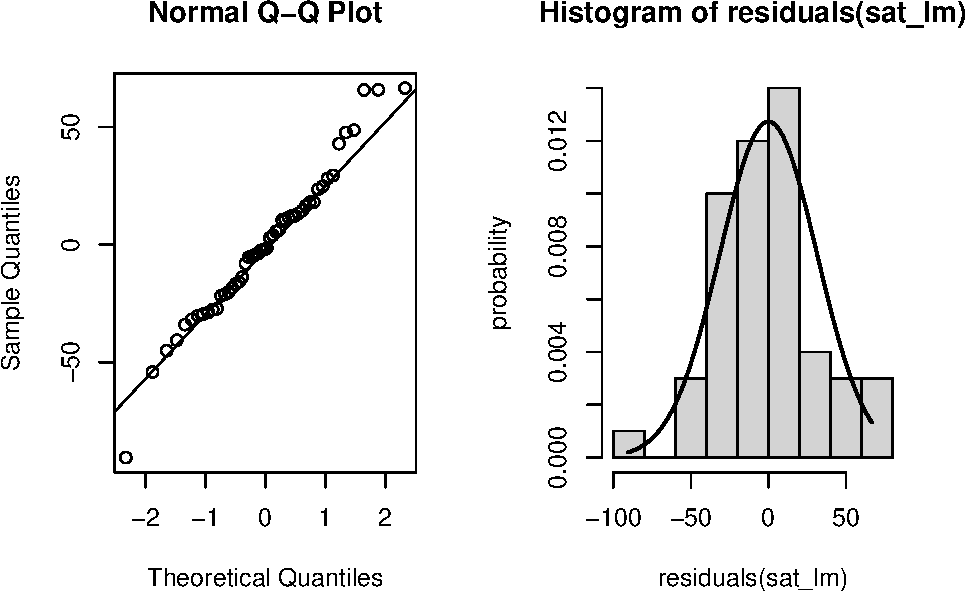
\includegraphics{AEII_main_files/figure-latex/unnamed-chunk-24-1.pdf}

\[
H_0:\ Os\ residuos\ seguem\ uma\ distribuic\tilde{a}o\ normal\
vs\
H_1:\ Os\ residuos\ n\tilde{a}o\ seguem\ uma\ distribuic\tilde{a}o\ normal
\]

\begin{Shaded}
\begin{Highlighting}[]
\FunctionTok{par}\NormalTok{(}\AttributeTok{mfrow =} \FunctionTok{c}\NormalTok{(}\DecValTok{1}\NormalTok{,}\DecValTok{1}\NormalTok{))}

\CommentTok{\# teste de Shapiro–Wilk}
\FunctionTok{shapiro.test}\NormalTok{(}\FunctionTok{residuals}\NormalTok{(sat\_lm))}
\end{Highlighting}
\end{Shaded}

\begin{verbatim}
## 
##  Shapiro-Wilk normality test
## 
## data:  residuals(sat_lm)
## W = 0.97691, p-value = 0.4304
\end{verbatim}

\(p-value = 0.4304 > 0.05 = \alpha\ \Rightarrow\ \) não rejeitamos
\(H_0\) para o nível de significância de 5\%, isto é, existe evidência
estatística de que os resíduos seguem uma distribuição normal.

Tendo em conta as representações gráficas, as mesmas reforçam a não
rejeição de \(H_0\), pelo facto dos resíduos exibirem uma grande
proximidade às linhas que representam a distribuição normal, em cada um
dos gráficos.

\(\ \)

Verifiquemos se o valor médio é zero e a variância constante:

\begin{Shaded}
\begin{Highlighting}[]
\FunctionTok{par}\NormalTok{(}\AttributeTok{mfrow =} \FunctionTok{c}\NormalTok{(}\DecValTok{1}\NormalTok{,}\DecValTok{2}\NormalTok{))}

\CommentTok{\# valor medio}
\FunctionTok{boxplot}\NormalTok{(}\FunctionTok{residuals}\NormalTok{(sat\_lm), }\AttributeTok{main =} \StringTok{"Residuals Scatter Plot"}\NormalTok{,}
     \AttributeTok{xlab =} \StringTok{"Observation"}\NormalTok{, }\AttributeTok{ylab =} \StringTok{"Residuals"}\NormalTok{)}
\FunctionTok{abline}\NormalTok{(}\AttributeTok{h =} \DecValTok{0}\NormalTok{, }\AttributeTok{col =} \StringTok{"black"}\NormalTok{, }\AttributeTok{lty =} \DecValTok{2}\NormalTok{)}

\CommentTok{\# homogeneidade de variancia}
\FunctionTok{plot}\NormalTok{(}\FunctionTok{fitted}\NormalTok{(sat\_lm), }\FunctionTok{rstandard}\NormalTok{(sat\_lm),}
     \AttributeTok{main =} \StringTok{"Standardized residuals vs Fitted"}\NormalTok{)}
\FunctionTok{abline}\NormalTok{(}\AttributeTok{h =} \DecValTok{0}\NormalTok{, }\AttributeTok{col =} \StringTok{"black"}\NormalTok{, }\AttributeTok{lty =} \DecValTok{2}\NormalTok{)}
\end{Highlighting}
\end{Shaded}

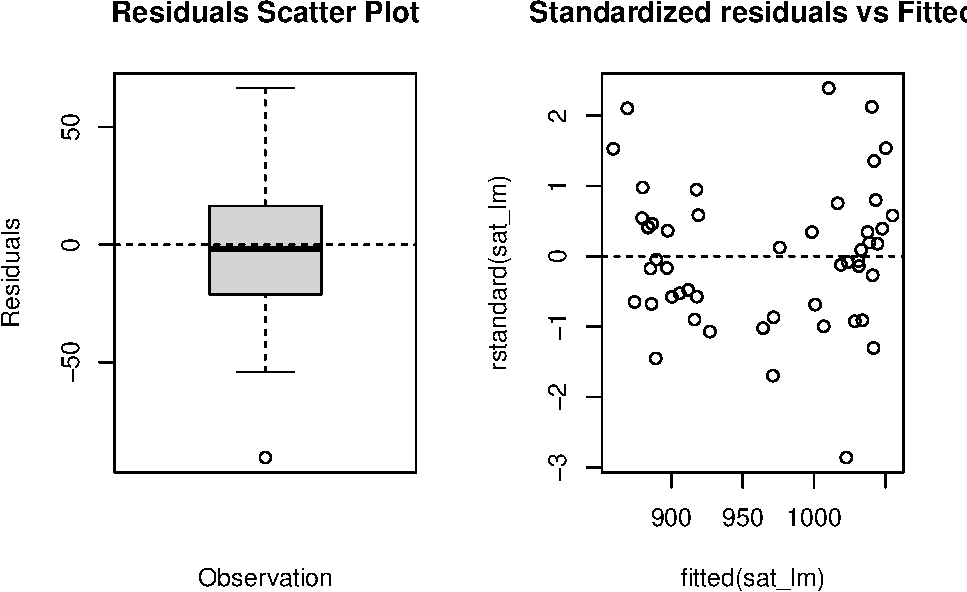
\includegraphics{AEII_main_files/figure-latex/unnamed-chunk-26-1.pdf}

\begin{Shaded}
\begin{Highlighting}[]
\FunctionTok{par}\NormalTok{(}\AttributeTok{mfrow =} \FunctionTok{c}\NormalTok{(}\DecValTok{1}\NormalTok{,}\DecValTok{1}\NormalTok{))}
\end{Highlighting}
\end{Shaded}

Repare-se que no primeiro gráfico podemos observar que a média dos
resíduos está muito próxima de zero, pelo que podemos afirmar que o
valor médio é zero. Para além disso, se recuarmos aos testes da
normalidade, podemos verificar no histograma que a linha com que os
resíduos têm uma grande proximidade representa uma distribuição normal
de valor médio zero, pelo que essa verificação já estava prevista.

Atendendo ao segundo gráfico, pelo facto dos pontos aparentarem estar
distribuídos de forma aleatória, em redor da linha horizonal que
representa o zero, temos a verificação de que estamos perante uma
variância constante.

\(\ \)

Analisemos, por fim, a independência:

\begin{Shaded}
\begin{Highlighting}[]
\CommentTok{\# carregar os pacotes, sem aviso de conflito}
\FunctionTok{library}\NormalTok{(zoo, }\AttributeTok{warn.conflicts =} \ConstantTok{FALSE}\NormalTok{)}
\FunctionTok{library}\NormalTok{(lmtest)}
\end{Highlighting}
\end{Shaded}

\[
H_0:\ \nexists\ autocorrelac\tilde{a}o\ nos\ residuos\
vs\
H_1:\ \exists\ autocorrelac\tilde{a}o\ nos\ residuos\
\]

\begin{Shaded}
\begin{Highlighting}[]
\CommentTok{\# teste de Durbin{-}Watson}
\FunctionTok{dwtest}\NormalTok{(sat\_lm)}
\end{Highlighting}
\end{Shaded}

\begin{verbatim}
## 
##  Durbin-Watson test
## 
## data:  sat_lm
## DW = 2.4525, p-value = 0.9459
## alternative hypothesis: true autocorrelation is greater than 0
\end{verbatim}

\(p-value = 0.9459 > 0.05 = \alpha\ \Rightarrow\ \) não rejeitamos
\(H_0\) para o nível de significância de 5\%, isto é, existe evidência
estatística de que não há autocorrelação nos resíduos, ou seja, há
independência entre eles.

\(\ \)

Podemos assim concluir, através das representações gráficas e dos testes
estatísticos realizados, que as suposições da regressão linear múltipla
se mantêm, pelo que o modelo parece ser apropriado para explicar a
relação entre as variáveis consideradas.

\subsection{Otimização do modelo: regressão stepwise}

Contudo, nada nos indica que o modelo que estimámos seja o ``melhor''
para explicar a pontuação média total no SAT (\emph{total}). Para testar
se existe um modelo ``melhor'', ou seja, um modelo que equilibre mais
adequadamente a sua complexidade e a explicação da variabilidade da
variável dependente, vamos utilizar a função \emph{step}
(\emph{stepwise}).

Ademais, devemos notar que a regressão \emph{stepwise}, dependendo do
modelo inicial e da direção escolhida, pode diferir. Assim sendo,
devemos partir de dois modelos diferentes e comparar as regressões
obtidas, pelo que optámos por partir de um modelo explicado por todas as
nossas variáveis (\(expend + ratio + salary + takers\)) e de um modelo
sem variáveis explicativas (\(1\)). Observemos o que acontece.

\begin{Shaded}
\begin{Highlighting}[]
\CommentTok{\# definir os modelos}
\NormalTok{min.model }\OtherTok{\textless{}{-}} \FunctionTok{lm}\NormalTok{(total }\SpecialCharTok{\textasciitilde{}} \DecValTok{1}\NormalTok{, }\AttributeTok{data =}\NormalTok{ sat\_clean)}
\NormalTok{max.model }\OtherTok{\textless{}{-}}\NormalTok{ sat\_lm}

\CommentTok{\# comeca com tudo mas pode tirar e meter}
\NormalTok{sat\_lm\_step.max }\OtherTok{\textless{}{-}} \FunctionTok{step}\NormalTok{(max.model, }\AttributeTok{direction =} \StringTok{"both"}\NormalTok{)}
\end{Highlighting}
\end{Shaded}

\begin{verbatim}
## Start:  AIC=353.48
## total ~ expend + ratio + salary + takers
## 
##          Df Sum of Sq    RSS    AIC
## - expend  1       191  48315 351.67
## - salary  1       503  48627 352.00
## - ratio   1      1359  49483 352.87
## <none>                 48124 353.48
## - takers  1    168688 216812 426.74
## 
## Step:  AIC=351.67
## total ~ ratio + salary + takers
## 
##          Df Sum of Sq    RSS    AIC
## <none>                 48315 351.67
## + expend  1       191  48124 353.48
## - ratio   1      5023  53338 354.62
## - salary  1      6782  55097 356.24
## - takers  1    171126 219441 425.34
\end{verbatim}

\begin{Shaded}
\begin{Highlighting}[]
\CommentTok{\# comeca sem nada mas pode meter e tirar}
\NormalTok{sat\_lm\_step.min }\OtherTok{\textless{}{-}} \FunctionTok{step}\NormalTok{(min.model, }\AttributeTok{direction =} \StringTok{"both"}\NormalTok{, }\AttributeTok{scope =} \FunctionTok{formula}\NormalTok{(max.model))}
\end{Highlighting}
\end{Shaded}

\begin{verbatim}
## Start:  AIC=432.5
## total ~ 1
## 
##          Df Sum of Sq    RSS    AIC
## + takers  1    215875  58433 357.18
## + salary  1     53078 221230 423.75
## + expend  1     39722 234586 426.68
## <none>                274308 432.50
## + ratio   1      1811 272497 434.17
## 
## Step:  AIC=357.18
## total ~ takers
## 
##          Df Sum of Sq    RSS    AIC
## + expend  1      8913  49520 350.91
## + salary  1      5095  53338 354.62
## + ratio   1      3336  55097 356.24
## <none>                 58433 357.18
## - takers  1    215875 274308 432.50
## 
## Step:  AIC=350.91
## total ~ takers + expend
## 
##          Df Sum of Sq    RSS    AIC
## <none>                 49520 350.91
## + ratio   1       893  48627 352.00
## + salary  1        38  49483 352.87
## - expend  1      8913  58433 357.18
## - takers  1    185066 234586 426.68
\end{verbatim}

Ao observarmos os resultados das regressões \emph{stepwise}, verificamos
que a escolha do modelo inicial teve impacto no modelo final obtido. Por
conseguinte, vamos criar um DataFrame para melhor comparar os dois
modelos estimados ao nosso modelo anterior.

\begin{Shaded}
\begin{Highlighting}[]
\NormalTok{sat.lm}\OtherTok{\textless{}{-}} \FunctionTok{c}\NormalTok{(}\FunctionTok{extractAIC}\NormalTok{(sat\_lm),}
              \FunctionTok{summary}\NormalTok{(sat\_lm)}\SpecialCharTok{$}\NormalTok{adj.r.squared)}
\NormalTok{step.max }\OtherTok{\textless{}{-}} \FunctionTok{c}\NormalTok{(}\FunctionTok{extractAIC}\NormalTok{(sat\_lm\_step.max),}
              \FunctionTok{summary}\NormalTok{(sat\_lm\_step.max)}\SpecialCharTok{$}\NormalTok{adj.r.squared)}
\NormalTok{step.min }\OtherTok{\textless{}{-}} \FunctionTok{c}\NormalTok{(}\FunctionTok{extractAIC}\NormalTok{(sat\_lm\_step.min),}
              \FunctionTok{summary}\NormalTok{(sat\_lm\_step.min)}\SpecialCharTok{$}\NormalTok{adj.r.squared)}
\NormalTok{step\_comparacao }\OtherTok{\textless{}{-}} \FunctionTok{data.frame}\NormalTok{(sat.lm, step.max, step.min)}
\FunctionTok{rownames}\NormalTok{(step\_comparacao) }\OtherTok{\textless{}{-}} \FunctionTok{c}\NormalTok{(}\StringTok{"Parameters"}\NormalTok{,}\StringTok{"AIC"}\NormalTok{,}\StringTok{"Adj. R\^{}2"}\NormalTok{)}
\NormalTok{step\_comparacao}
\end{Highlighting}
\end{Shaded}

\begin{verbatim}
##                 sat.lm    step.max    step.min
## Parameters   5.0000000   4.0000000   3.0000000
## AIC        353.4755564 351.6740977 350.9055047
## Adj. R^2     0.8089679   0.8123772   0.8117906
\end{verbatim}

Através da análise do DataFrame criado, podemos verificar que, em
relação ao modelo anterior, os dois novos modelos estimados têm menos
parâmetros a estimar, um menor AIC e uma melhor explicação sobre a
variação da variável \emph{total}.

Comparando os dois novos modelos, verificamos que o modelo
\emph{step.min}, para além de ter menos parâmetros a estimar e um menor
AIC, explica aproximadamente 81.2\% da variação da variável
\emph{total}, tal como o modelo \emph{step.max}.

Desta forma, podemos concluir que o modelo mais adequado para explicar a
pontuação média total no SAT (\emph{total}) é o seguinte:

\begin{Shaded}
\begin{Highlighting}[]
\NormalTok{sat\_lm.step }\OtherTok{\textless{}{-}}\NormalTok{ sat\_lm\_step.min}
\NormalTok{sat\_lm.step}
\end{Highlighting}
\end{Shaded}

\begin{verbatim}
## 
## Call:
## lm(formula = total ~ takers + expend, data = sat_clean)
## 
## Coefficients:
## (Intercept)       takers       expend  
##     993.832       -2.851       12.287
\end{verbatim}

\subsection{Confirmação do modelo ótimo: testes F-parciais}

Uma vez obtido o novo modelo, através do método \emph{stepwise}, podemos
confirmar as escolhas das variáveis incluídas no mesmo, através de
testes F-parciais. A realização de testes F-parciais vai-nos permitir
avaliar se a inclusão de variáveis específicas no modelo melhora
significativamente a explicação da variabilidade da variável dependente,
ou não.

De modo a facilitar a realização dos testes F-parciais, vamos criar uma
função que os realize entre um modelo inicial e vários modelos com
apenas mais uma variável que o inicial e, de seguida, apresente o
p-value associado a cada um dos testes.

\begin{Shaded}
\begin{Highlighting}[]
\NormalTok{testes\_f\_parcial }\OtherTok{\textless{}{-}} \ControlFlowTok{function}\NormalTok{(formula\_0, variaveis) \{}
  \CommentTok{\# modelo inicial}
\NormalTok{  modelo\_0 }\OtherTok{\textless{}{-}} \FunctionTok{lm}\NormalTok{(}\FunctionTok{as.formula}\NormalTok{(formula\_0), }\AttributeTok{data =}\NormalTok{ sat\_clean)}
  
  \CommentTok{\# fazer anova com a adicao de cada variavel}
\NormalTok{  resultados\_anova }\OtherTok{\textless{}{-}} \FunctionTok{lapply}\NormalTok{(variaveis, }\ControlFlowTok{function}\NormalTok{(x) \{}
\NormalTok{    formula\_i }\OtherTok{\textless{}{-}} \FunctionTok{paste}\NormalTok{(formula\_0, }\StringTok{"+"}\NormalTok{, x)}
\NormalTok{    modelo\_i }\OtherTok{\textless{}{-}} \FunctionTok{lm}\NormalTok{(}\FunctionTok{as.formula}\NormalTok{(formula\_i), }\AttributeTok{data =}\NormalTok{ sat\_clean)}
    \FunctionTok{anova}\NormalTok{(modelo\_0, modelo\_i)\})}
  
  \CommentTok{\# selecionar os p{-}values}
\NormalTok{  p\_values }\OtherTok{\textless{}{-}} \FunctionTok{sapply}\NormalTok{(resultados\_anova, }\ControlFlowTok{function}\NormalTok{(resultado) resultado}\SpecialCharTok{$}\StringTok{"Pr(\textgreater{}F)"}\NormalTok{[}\DecValTok{2}\NormalTok{])}
  
  \CommentTok{\# criar dataframe para melhorar a visualizacao}
\NormalTok{  df }\OtherTok{\textless{}{-}} \FunctionTok{t}\NormalTok{(p\_values)}
  \FunctionTok{colnames}\NormalTok{(df) }\OtherTok{\textless{}{-}}\NormalTok{ variaveis}
  \FunctionTok{rownames}\NormalTok{(df) }\OtherTok{\textless{}{-}} \FunctionTok{c}\NormalTok{(}\StringTok{"p{-}values"}\NormalTok{)}
  
  \FunctionTok{return}\NormalTok{(df)}
\NormalTok{\}}
\end{Highlighting}
\end{Shaded}

Note-se que os testes têm as seguintes hipóteses associadas: \[
H_0:\ A\ vari\acute{a}vel\ x_i\ n\tilde{a}o\ \acute{e}\ significativa\ para\ o\ modelo\
vs\
H_1:\ A\ vari\acute{a}vel\ x_i\ \acute{e}\ significativa\ para\ o\ modelo
\]

Comecemos com um modelo inicial sem variáveis explicativas e comparemos
com os modelos que contêm cada uma destas.

\begin{Shaded}
\begin{Highlighting}[]
\FunctionTok{testes\_f\_parcial}\NormalTok{(}\StringTok{"total \textasciitilde{} 1"}\NormalTok{, }\FunctionTok{c}\NormalTok{(}\StringTok{"expend"}\NormalTok{, }\StringTok{"salary"}\NormalTok{, }\StringTok{"ratio"}\NormalTok{, }\StringTok{"takers"}\NormalTok{))}
\end{Highlighting}
\end{Shaded}

\begin{verbatim}
##               expend     salary     ratio       takers
## p-values 0.006407965 0.00139131 0.5748329 9.791875e-18
\end{verbatim}

Como podemos observar, os p-values associados às variáveis
\emph{expend}, \emph{salary} e \emph{takers} são menores que 5\%, o
nosso nível de significância, pelo que rejeitamos os \(H_0\) associados
a estas variáveis. Isto é, existe evidência estatística de que cada uma
destas variáveis é significativa para o seu modelo.

Contudo, como o menor p-value é o associado à variável \emph{takers},
vamos realizar novamente os testes F-parciais, mas desta vez adicionando
a variável \emph{takers} ao modelo incial e comparemos com os modelos
idênticos a este, mas com a adição de cada uma das restantes variáveis.

\begin{Shaded}
\begin{Highlighting}[]
\FunctionTok{testes\_f\_parcial}\NormalTok{(}\StringTok{"total \textasciitilde{} takers"}\NormalTok{, }\FunctionTok{c}\NormalTok{(}\StringTok{"expend"}\NormalTok{, }\StringTok{"salary"}\NormalTok{, }\StringTok{"ratio"}\NormalTok{))}
\end{Highlighting}
\end{Shaded}

\begin{verbatim}
##               expend     salary      ratio
## p-values 0.005529458 0.03942052 0.09823538
\end{verbatim}

Analogamente, adicionemos agora a variável \emph{expend}.

\begin{Shaded}
\begin{Highlighting}[]
\FunctionTok{testes\_f\_parcial}\NormalTok{(}\StringTok{"total \textasciitilde{} takers + expend"}\NormalTok{, }\FunctionTok{c}\NormalTok{(}\StringTok{"salary"}\NormalTok{, }\StringTok{"ratio"}\NormalTok{))}
\end{Highlighting}
\end{Shaded}

\begin{verbatim}
##             salary     ratio
## p-values 0.8526704 0.3629065
\end{verbatim}

\(min\{p-values\} \approx 0.3629 > 0.05 = \alpha\ \Rightarrow\ \) não
rejeitamos nenhum dos \(H_0\) para o nível de significância de 5\%, isto
é, existe evidência estatística de que o modelo mais simples, ou seja,
aquele que só tem como variáveis explicativas as variáveis \emph{takers}
e \emph{expend}, é suficiente para explicar a variável dependente
(\emph{total}).

Com isto, podemos reparar que o ``melhor'' modelo obtido, tendo por base
os critérios utilizados nestes testes F-parciais, é idêntico ao
``melhor'' modelo obtido através do método \emph{stepwise}, o que
reforça a validade e consistência do modelo estimado.

\subsection{Análise do modelo ótimo}

Por fim, analisemos o modelo de regressão linear múltipla que obtemos
através da otimização do modelo inicial.

\(\ \)

Comecemos por analisar as variáveis do modelo:

\begin{Shaded}
\begin{Highlighting}[]
\FunctionTok{summary}\NormalTok{(sat\_lm.step)}\SpecialCharTok{$}\NormalTok{call}
\end{Highlighting}
\end{Shaded}

\begin{verbatim}
## lm(formula = total ~ takers + expend, data = sat_clean)
\end{verbatim}

\begin{Shaded}
\begin{Highlighting}[]
\FunctionTok{summary}\NormalTok{(sat\_lm.step)}\SpecialCharTok{$}\NormalTok{coefficients}
\end{Highlighting}
\end{Shaded}

\begin{verbatim}
##               Estimate Std. Error    t value     Pr(>|t|)
## (Intercept) 993.831659 21.8332335  45.519215 1.579349e-40
## takers       -2.850929  0.2151123 -13.253212 1.729825e-17
## expend       12.286518  4.2243159   2.908523 5.529458e-03
\end{verbatim}

Podemos observar que o modelo, como vimos anteriormente, tem como
variáveis explicativas as despesas (\emph{expend}) e a percentagem de
alunos elegíveis para fazerem o exame (\emph{takers}) e como variável
dependente a pontuação média total no SAT (\emph{total}).

Para além disso, podemos observar que os coeficientes \(\beta_0\),
\(\beta_{takers}\) e \(\beta_{expend}\) são agora, aproximadamente,
993.83, -2.85 e 12.29, respetivamente, e que
\(max\{p-value\} \approx 5.53e-03 < 0.05 = \alpha\ \Rightarrow\ \) para
um nível de significância de 5\%, existe evidência estatística de que
cada uma das variáveis é significativa para o modelo.

\(\ \)

Verifiquemos agora a significância do modelo através do cálculo do
p-value, ao invés da sua observação direta, com o objetivo de explorar
mais funções do R: \[
H_0:\ \beta_0=\beta_{takers}=\beta_{expend}=0\
vs\
H_1:\ \exists_i:\beta_i \neq 0
\]

\begin{Shaded}
\begin{Highlighting}[]
\NormalTok{fstatistic\_value }\OtherTok{\textless{}{-}} \FunctionTok{summary}\NormalTok{(sat\_lm.step)}\SpecialCharTok{$}\NormalTok{fstatistic[}\DecValTok{1}\NormalTok{] }\CommentTok{\# = 106.7}
\NormalTok{fstatistic\_numdf }\OtherTok{\textless{}{-}} \FunctionTok{summary}\NormalTok{(sat\_lm.step)}\SpecialCharTok{$}\NormalTok{fstatistic[}\DecValTok{2}\NormalTok{] }\CommentTok{\# = 2}
\NormalTok{fstatistic\_dendf }\OtherTok{\textless{}{-}} \FunctionTok{summary}\NormalTok{(sat\_lm.step)}\SpecialCharTok{$}\NormalTok{fstatistic[}\DecValTok{3}\NormalTok{] }\CommentTok{\# = 47}

\FunctionTok{pf}\NormalTok{(fstatistic\_value, fstatistic\_numdf, fstatistic\_dendf, }\AttributeTok{lower.tail =} \ConstantTok{FALSE}\NormalTok{)}
\end{Highlighting}
\end{Shaded}

\begin{verbatim}
##        value 
## 3.378819e-18
\end{verbatim}

\(p-value = 3.378819e-18 < 0.05 = \alpha\ \Rightarrow\ \) rejeitamos
\(H_0\) para o nível de significância de 5\%, isto é, existe evidência
estatística de que o modelo ajustado é significativo, ou seja, pelo
menos uma das variáveis explicativas tem um efeito significativo sobre a
variável dependente.

\(\ \)

De seguida, criemos gráficos de resíduos \emph{vs} fatores, com o
objetivo de observar se existem, ou não, padrões na dispersão dos
resíduos, consoante a variável explicativa.

\begin{Shaded}
\begin{Highlighting}[]
\FunctionTok{par}\NormalTok{(}\AttributeTok{mfrow =} \FunctionTok{c}\NormalTok{(}\DecValTok{1}\NormalTok{, }\DecValTok{2}\NormalTok{))}

\CommentTok{\# residuos vs takers}
\FunctionTok{plot}\NormalTok{(sat\_clean}\SpecialCharTok{$}\NormalTok{takers, }\FunctionTok{residuals}\NormalTok{(sat\_lm.step), }
     \AttributeTok{xlab =} \StringTok{"takers"}\NormalTok{, }\AttributeTok{ylab =} \StringTok{"Residuals"}\NormalTok{,}
     \AttributeTok{main =} \StringTok{"Residuals vs takers"}\NormalTok{)}

\CommentTok{\# residuos vs expend}
\FunctionTok{plot}\NormalTok{(sat\_clean}\SpecialCharTok{$}\NormalTok{expend, }\FunctionTok{residuals}\NormalTok{(sat\_lm.step), }
     \AttributeTok{xlab =} \StringTok{"expend"}\NormalTok{, }\AttributeTok{ylab =} \StringTok{"Residuals"}\NormalTok{,}
     \AttributeTok{main =} \StringTok{"Residuals vs expend"}\NormalTok{)}
\end{Highlighting}
\end{Shaded}

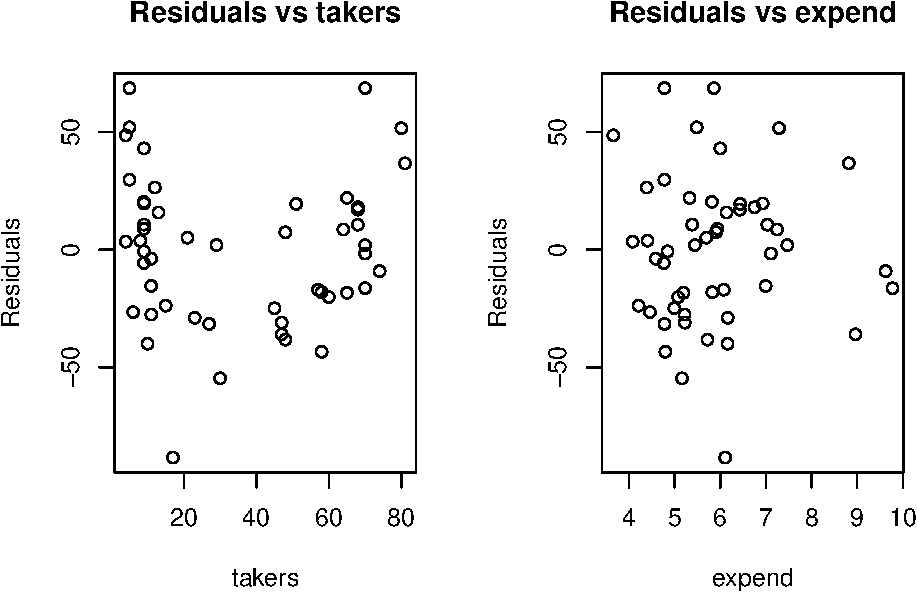
\includegraphics{AEII_main_files/figure-latex/unnamed-chunk-38-1.pdf}

\begin{Shaded}
\begin{Highlighting}[]
\FunctionTok{par}\NormalTok{(}\AttributeTok{mfrow =} \FunctionTok{c}\NormalTok{(}\DecValTok{1}\NormalTok{, }\DecValTok{1}\NormalTok{))}
\end{Highlighting}
\end{Shaded}

Verifica-se a inexistência de padrões na distribuição dos resíduos, o
que nos sugere que o modelo consegue explicar as variações da variável
dependente de forma consistente, ao longo dos diferentes níveis dos
fatores.

\(\ \)

Relembremos que é de elevada importância a verificação de certas
condições para que o modelo seja aplicável e que os seus resultados
possam ser interpretados de maneira significativa. Verifiquemos as
seguintes condições:

\begin{Shaded}
\begin{Highlighting}[]
\FunctionTok{library}\NormalTok{(performance, }\AttributeTok{warn.conflicts =} \ConstantTok{FALSE}\NormalTok{)}
\FunctionTok{check\_model}\NormalTok{(sat\_lm.step)}
\end{Highlighting}
\end{Shaded}

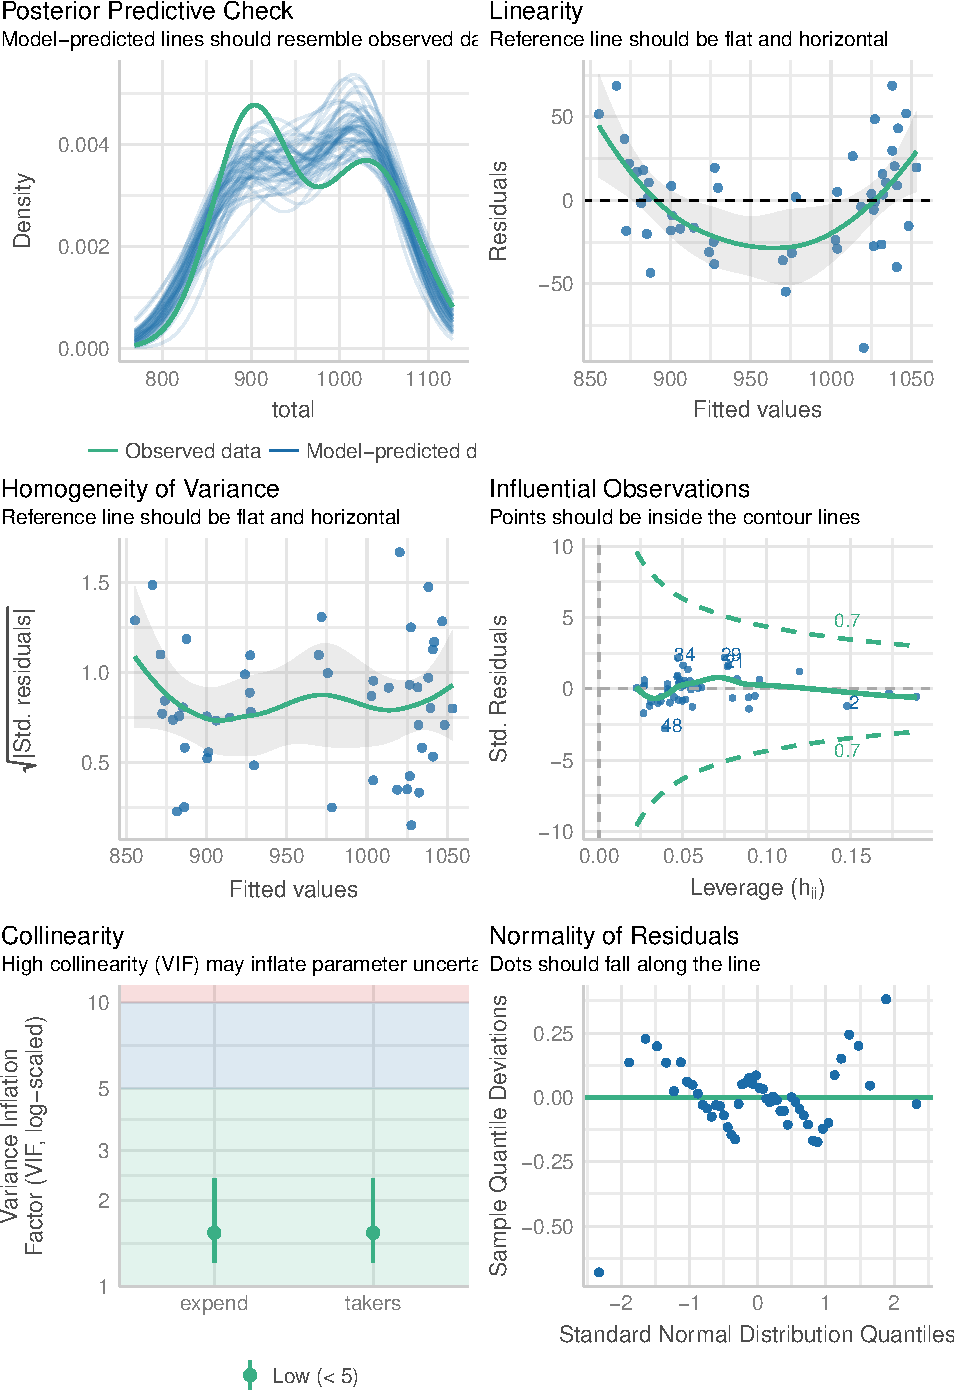
\includegraphics{AEII_main_files/figure-latex/unnamed-chunk-39-1.pdf}

\emph{Posterior Predictive Check}: podemos verificar que não existem
discrepâncias significativas entre os dados reais e os simulados, pelo
que podemos afirmar que o modelo se ajusta bem aos dados.

\emph{Linearity}: devemos notar que a linha que melhor se ajusta aos
pontos não é completamente horizontal, mas também não se assemelha
significativamente a um ``U''. Isto indica-nos que a relação entre as
variáveis pode não ser linear.

\emph{Homogeneity of Variance}: notemos que a linha é aproximadamente
horizontal, pelo que será expectável que haja homogeneidade de
variâncias.

\emph{Influential Observations}: verifiquemos que os pontos estão todos
dentro das linhas a tracejado, pelo que as distâncias de Cook (analisam
o impacto de cada ponto de dados na estimação dos coeficientes do modelo
de regressão, o que acaba por ser uma verificação de outliers) são
respeitadas.

\emph{Collinearity}: podemos verificar que o VIF é baixo para ambas as
variáveis, o que nos indica que não há correlação significativa entre
elas.

\emph{Normality of Residuals}: notemos que os pontos, de forma
significativa, alinham-se ao longo da linha horizontal, o que nos
permite afirmar que os resíduos têm uma distribuição normal.

\(\ \)

Para finalizar, vamos criar um gráfico 3D que compare os valores
estimados pelo modelo de regressão linear estimado, face aos valores
reais do conjunto de dados.

\begin{Shaded}
\begin{Highlighting}[]
\FunctionTok{library}\NormalTok{(scatterplot3d)}

\NormalTok{x\_min }\OtherTok{\textless{}{-}} \FunctionTok{min}\NormalTok{(sat\_clean}\SpecialCharTok{$}\NormalTok{takers) }\SpecialCharTok{*} \FloatTok{0.9}
\NormalTok{x\_max }\OtherTok{\textless{}{-}} \FunctionTok{max}\NormalTok{(sat\_clean}\SpecialCharTok{$}\NormalTok{takers) }\SpecialCharTok{*} \FloatTok{1.1}
\NormalTok{y\_min }\OtherTok{\textless{}{-}} \FunctionTok{min}\NormalTok{(sat\_clean}\SpecialCharTok{$}\NormalTok{expend) }\SpecialCharTok{*} \FloatTok{0.9}
\NormalTok{y\_max }\OtherTok{\textless{}{-}} \FunctionTok{max}\NormalTok{(sat\_clean}\SpecialCharTok{$}\NormalTok{expend) }\SpecialCharTok{*} \FloatTok{1.1}

\NormalTok{predictions }\OtherTok{\textless{}{-}} \FunctionTok{predict}\NormalTok{(sat\_lm.step,}
                       \AttributeTok{newdata =} \FunctionTok{data.frame}\NormalTok{(}\AttributeTok{takers =} \FunctionTok{c}\NormalTok{(x\_min, x\_max),}
                                            \AttributeTok{expend =} \FunctionTok{c}\NormalTok{(y\_min, y\_max)))}

\NormalTok{sat\_lm.graph }\OtherTok{\textless{}{-}} \FunctionTok{scatterplot3d}\NormalTok{(}\FunctionTok{c}\NormalTok{(x\_min,x\_max), }\FunctionTok{c}\NormalTok{(y\_min,y\_max), predictions,}
                     \AttributeTok{color =} \StringTok{"black"}\NormalTok{, }\AttributeTok{type =} \StringTok{"l"}\NormalTok{, }\AttributeTok{angle =} \DecValTok{30}\NormalTok{,}
                     \AttributeTok{xlab =} \StringTok{"takers"}\NormalTok{, }\AttributeTok{ylab =} \StringTok{"expend"}\NormalTok{, }\AttributeTok{zlab =} \StringTok{"total"}\NormalTok{,}
                     \AttributeTok{zlim =} \FunctionTok{c}\NormalTok{(}\FunctionTok{min}\NormalTok{(sat\_clean}\SpecialCharTok{$}\NormalTok{total)}\SpecialCharTok{*}\FloatTok{0.9}\NormalTok{, }\FunctionTok{max}\NormalTok{(sat\_clean}\SpecialCharTok{$}\NormalTok{total)}\SpecialCharTok{*}\FloatTok{1.1}\NormalTok{),}
                     \AttributeTok{main =} \StringTok{"Regressão sat\_lm.step"}\NormalTok{, }\AttributeTok{cex.axis =} \FloatTok{0.6}\NormalTok{)}

\NormalTok{sat\_lm.graph}\SpecialCharTok{$}\FunctionTok{points3d}\NormalTok{(sat\_clean}\SpecialCharTok{$}\NormalTok{takers, sat\_clean}\SpecialCharTok{$}\NormalTok{expend, sat\_clean}\SpecialCharTok{$}\NormalTok{total,}
             \AttributeTok{col =} \StringTok{"darkgray"}\NormalTok{, }\AttributeTok{type =} \StringTok{"p"}\NormalTok{)}
\end{Highlighting}
\end{Shaded}

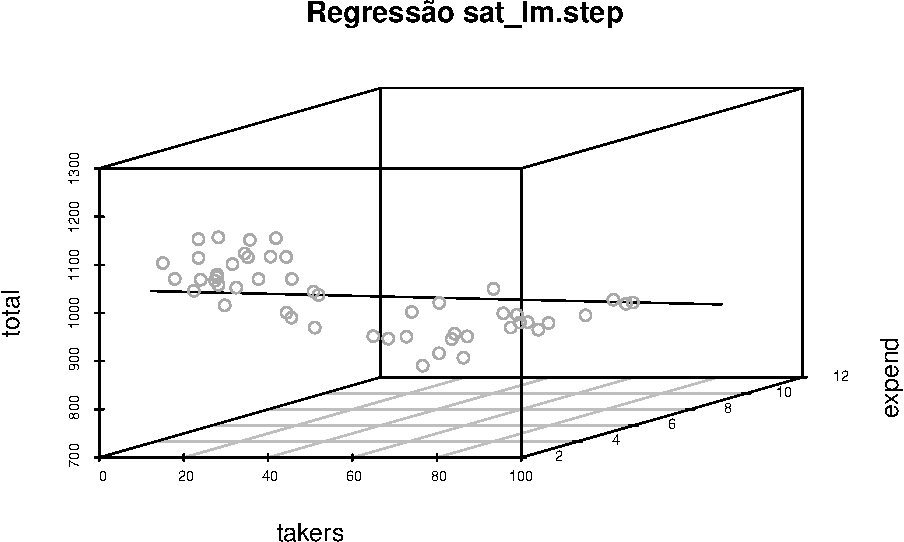
\includegraphics{AEII_main_files/figure-latex/unnamed-chunk-40-1.pdf}

\newpage
\section{Conclusão}

A realização deste trabalho deu-nos a oportunidade de explorar mais
aprofundadamente as linguagens Rmarkdown e R, tal como o software
RStudio. Ademais, através da utlização do R, conseguimos percecionar, em
primeira mão, a grande assistência que o mesmo oferece durante a análise
de conjuntos de dados, revelando-se particularmente crucial no contexo
estatístico.

\(\ \)

No âmbito específico da análise de variância, o R destaca-se pela sua
capacidade de realizar uma avaliação abrangente das diferenças entre
grupos. Além de identificar variações significativas entre médias, o R
disponibiliza ferramentas integradas para a verificação de pressupostos
essencias, tanto de forma numérica como visual, reforçando a validação
dos resultados obtidos na análise de variância.

\(\ \)

Quanto à regressão linear múltipla, a linguagem de programação
permite-nos explorar relações entre variáveis, identificar padrões,
testar pressupostos sobre as observações e, ainda, comparar diferentes
modelos explicativos, o que inclui a flexiblidade para combinar
diferentes conjuntos de variáveis explicativas, possiblitando a
identificação do modelo que melhor se adequa ao conjunto de dados.

\(\ \)

Em suma, este trabalho não apenas aprofundou o nosso conhecimento
estatístico, como também ressaltou a importância da utlização de
ferramentas computacionais no âmbito da análise estatística.


\end{document}
